\begin{figure}[!htbp]
\begin{center}
  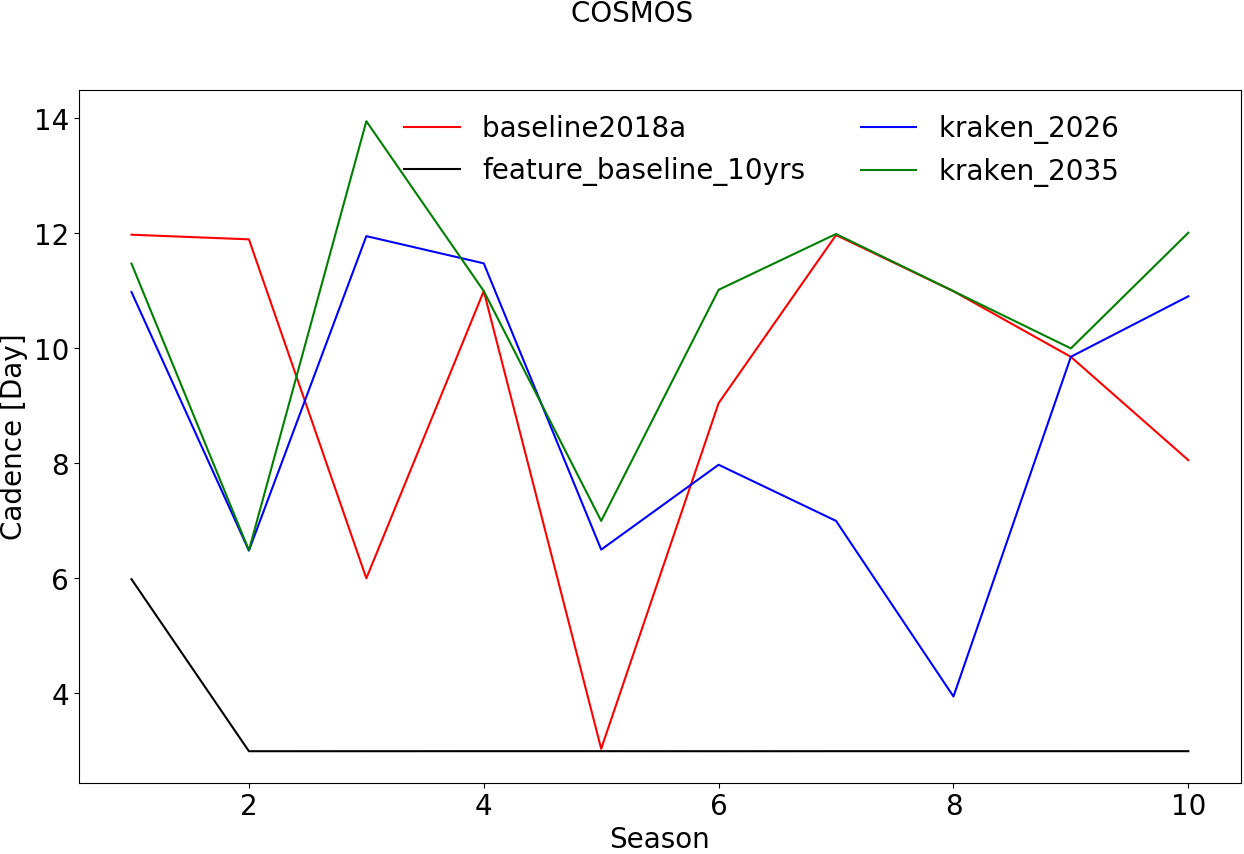
\includegraphics[width=9cm]{overview_strategy/COSMOS_cadence.png}
  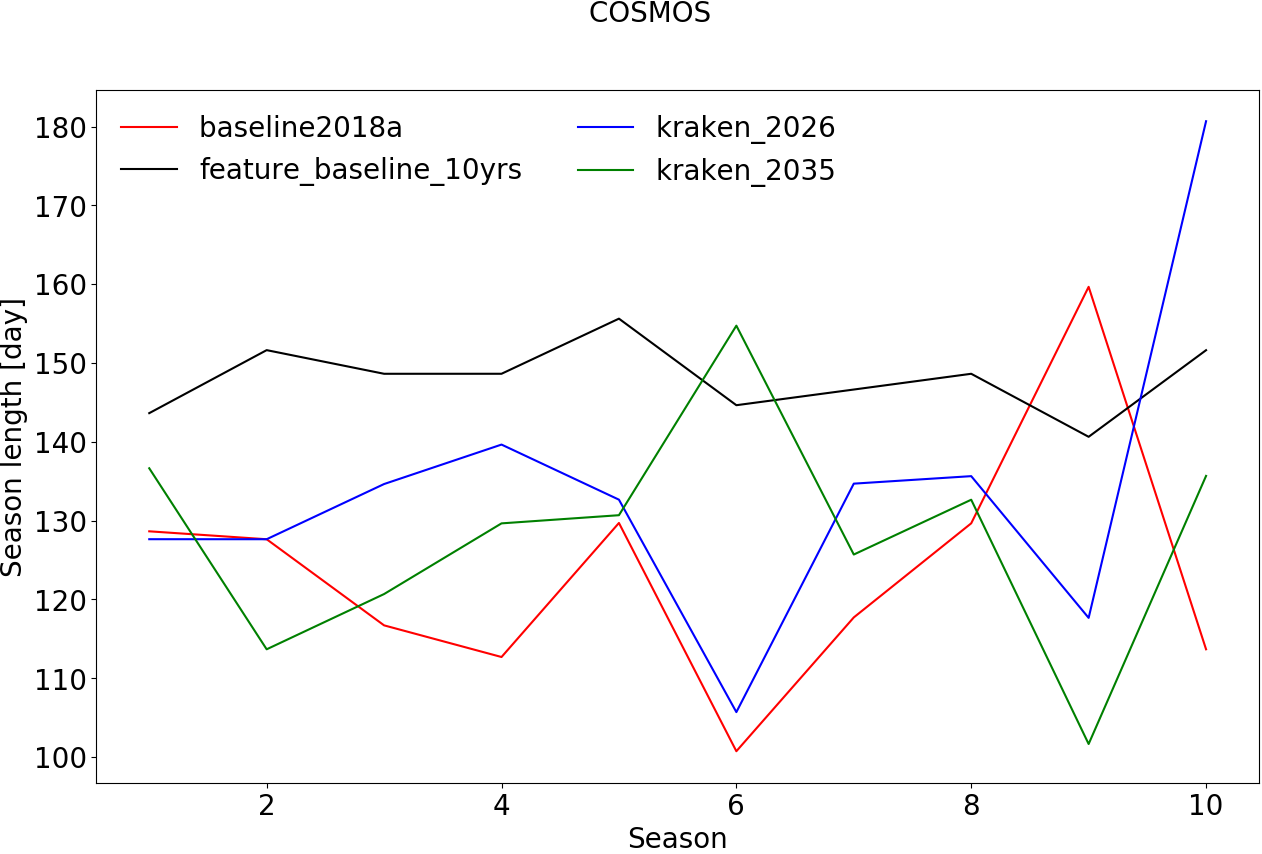
\includegraphics[width=9cm]{overview_strategy/COSMOS_season_length.png}
  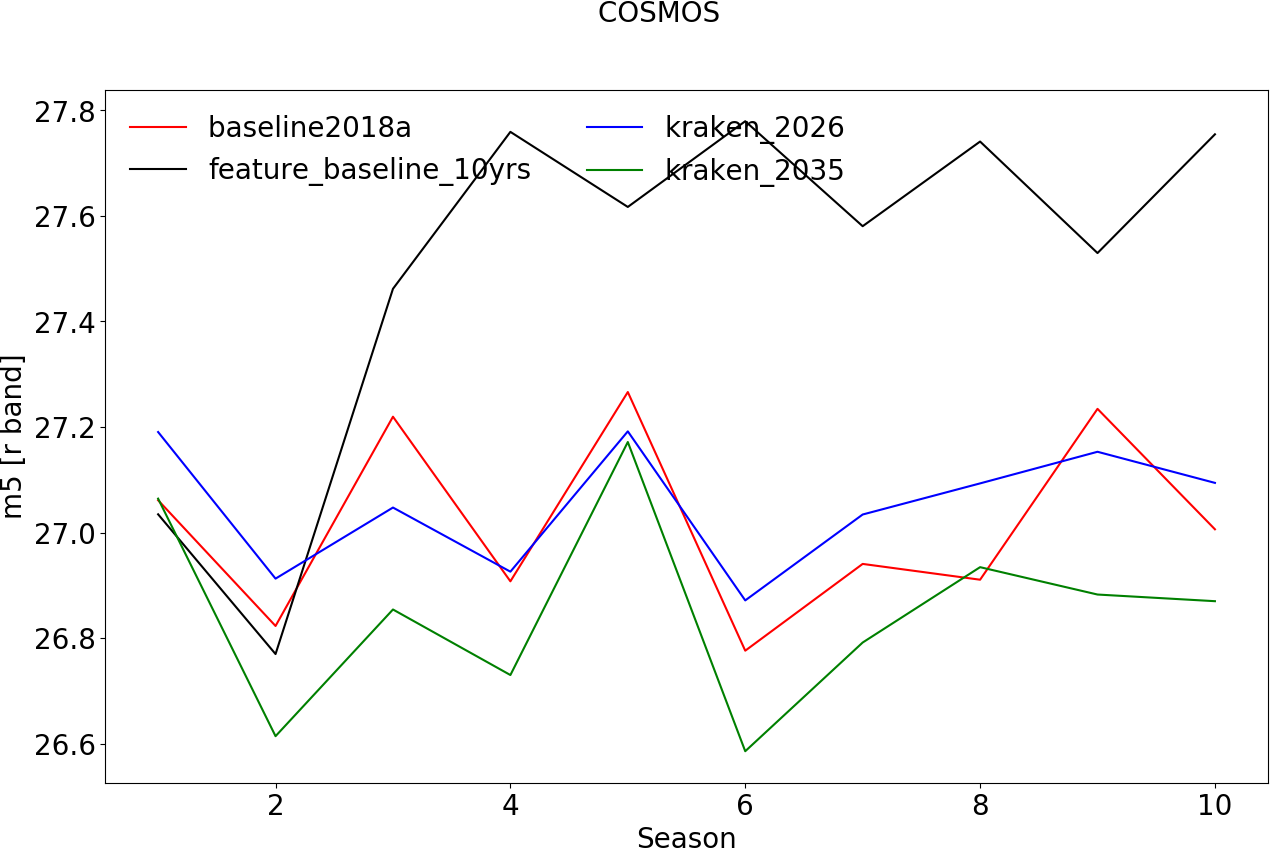
\includegraphics[width=9cm]{overview_strategy/COSMOS_m5.png}
  %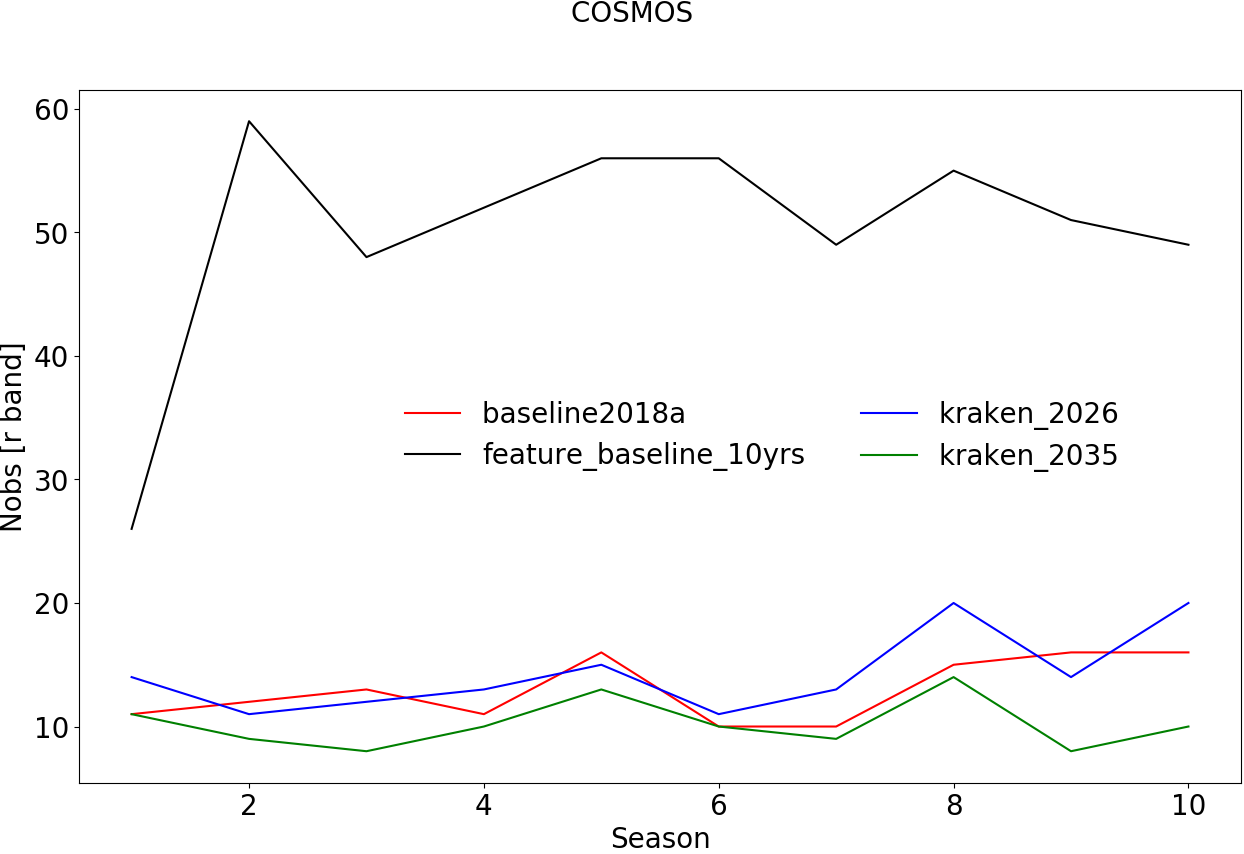
\includegraphics[width=9cm]{overview_strategy/COSMOS_Nobs.png}
 \caption{Cadence (top, in day), season length (middle, in day) and coadded m5 (bottom, in mag) as a function of the season for the COSMOS field and baseline18a, feature\_baseline\_10yrs, kralen\_2026 and kraken\_2035 observing strategies.}\label{fig:cosmoscad}
\end{center}
\end{figure}

\begin{figure}[!htbp]
\begin{center}
  
  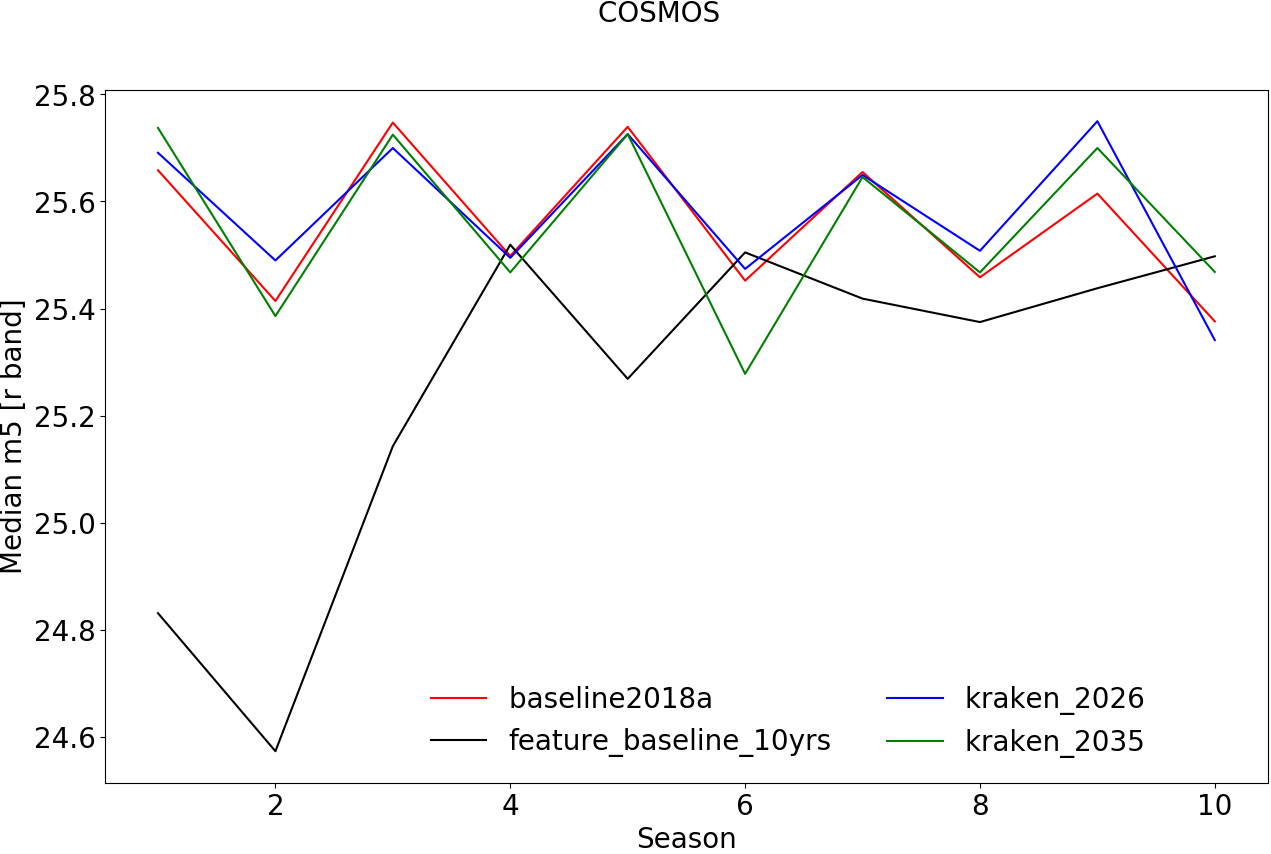
\includegraphics[width=9cm]{overview_strategy/COSMOS_med_m5.png}
  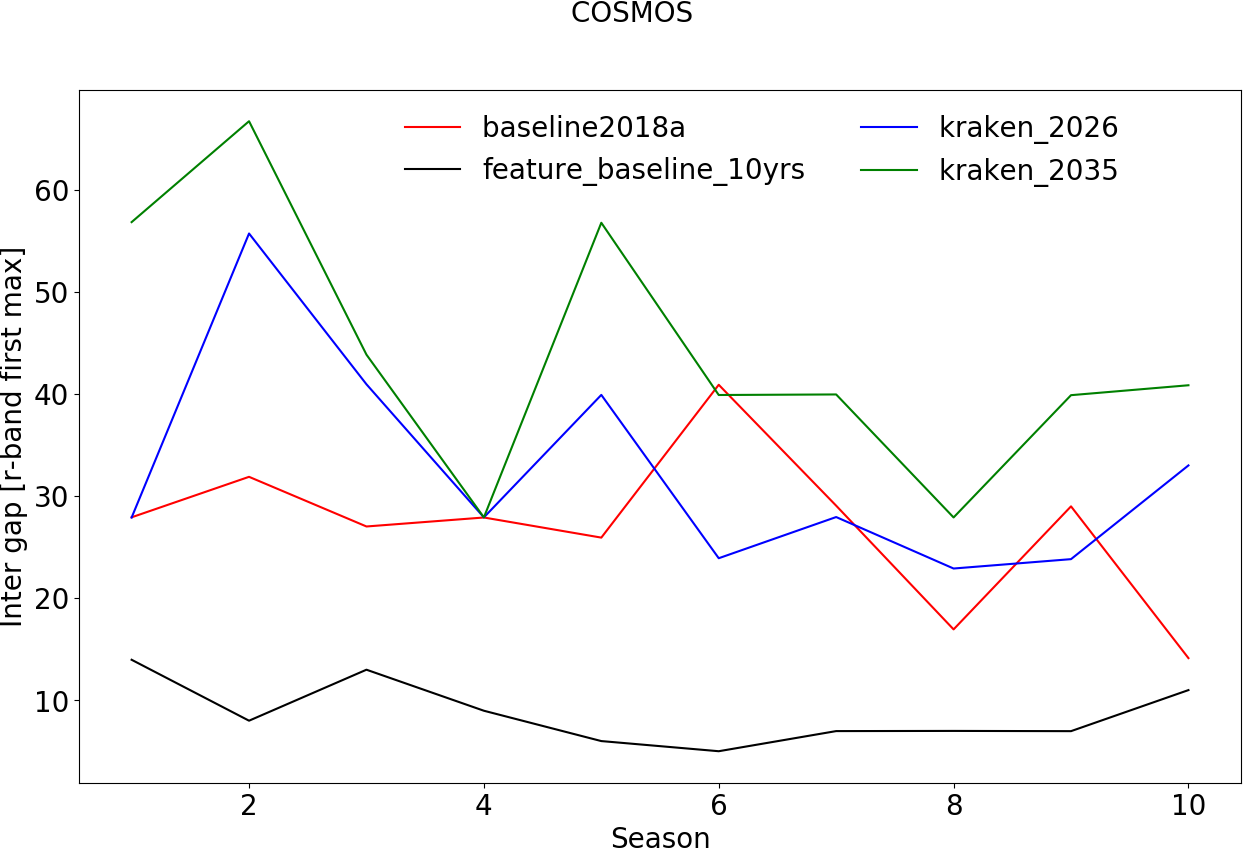
\includegraphics[width=9cm]{overview_strategy/COSMOS_intergap_max1.png}
    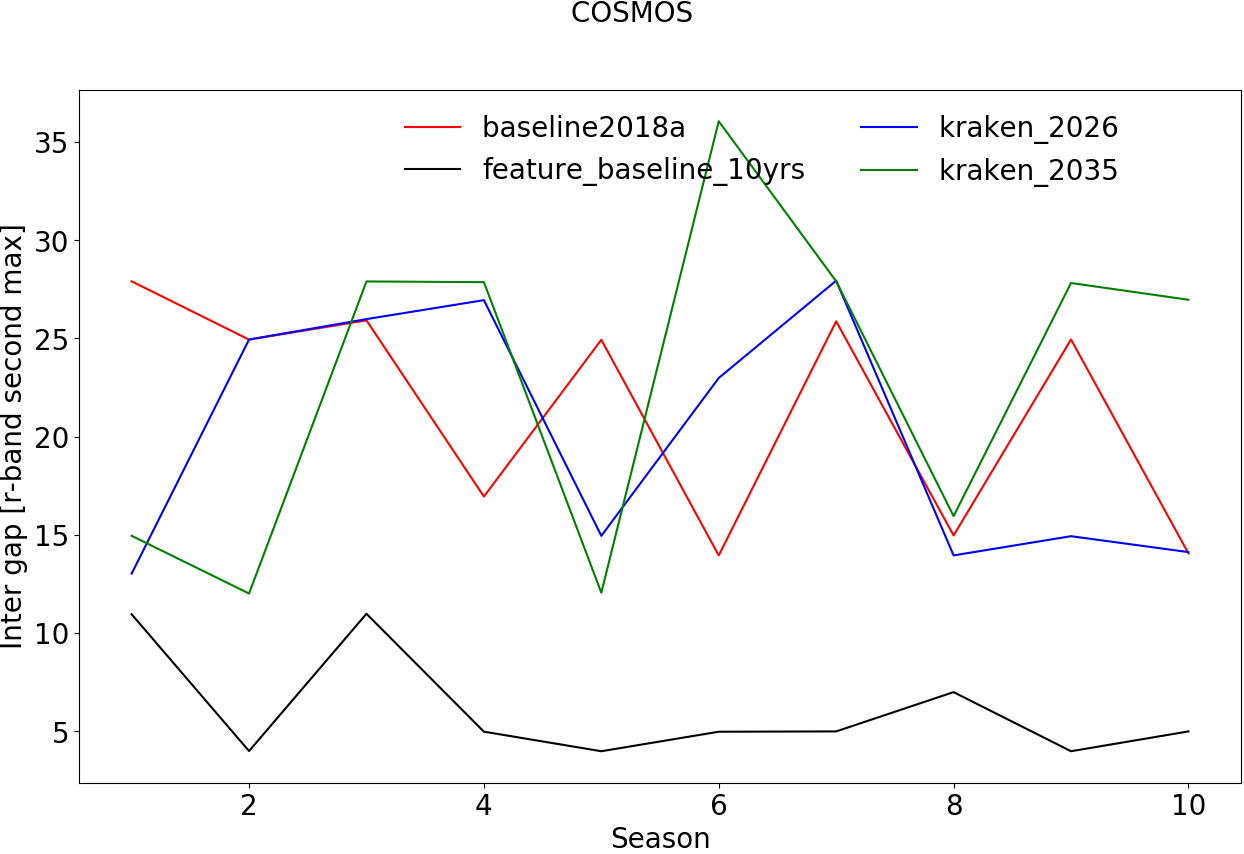
\includegraphics[width=9cm]{overview_strategy/COSMOS_intergap_max2.png}
 \caption{Median m5 (top, in mag), first maximum inter-night gap (middle, in day) and second maximum inter-night gap (bottom, in day)  as a function of the season for the COSMOS field and baseline18a, feature\_baseline\_10yrs, kralen\_2026 and kraken\_2035 observing strategies.}\label{fig:cosmos_m5}
\end{center}
\end{figure}

%%%%%%%%%%%%%%%%%%%%%%%%%%%%%%%%%%%%%%%%%%%%%%


\begin{figure}[!htbp]
\begin{center}
  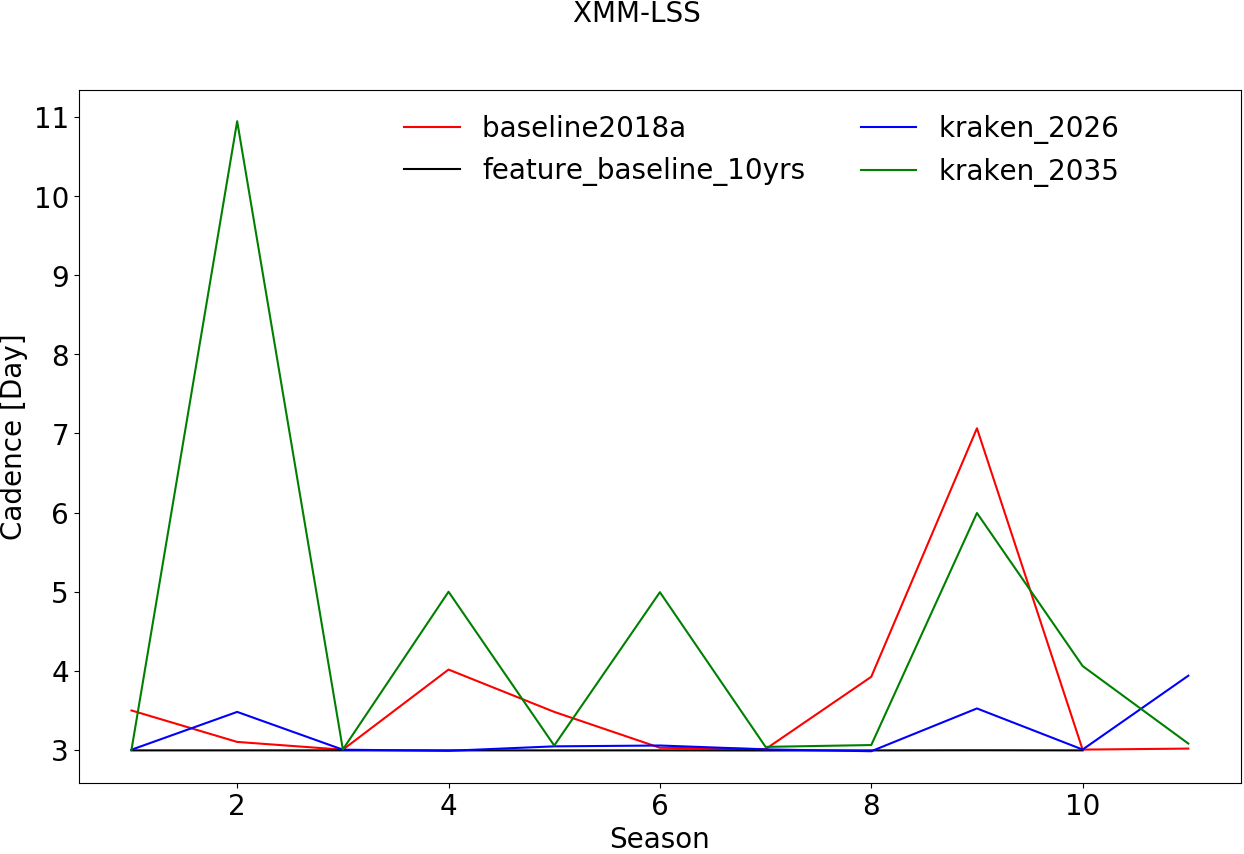
\includegraphics[width=9cm]{overview_strategy/XMM-LSS_cadence.png}
  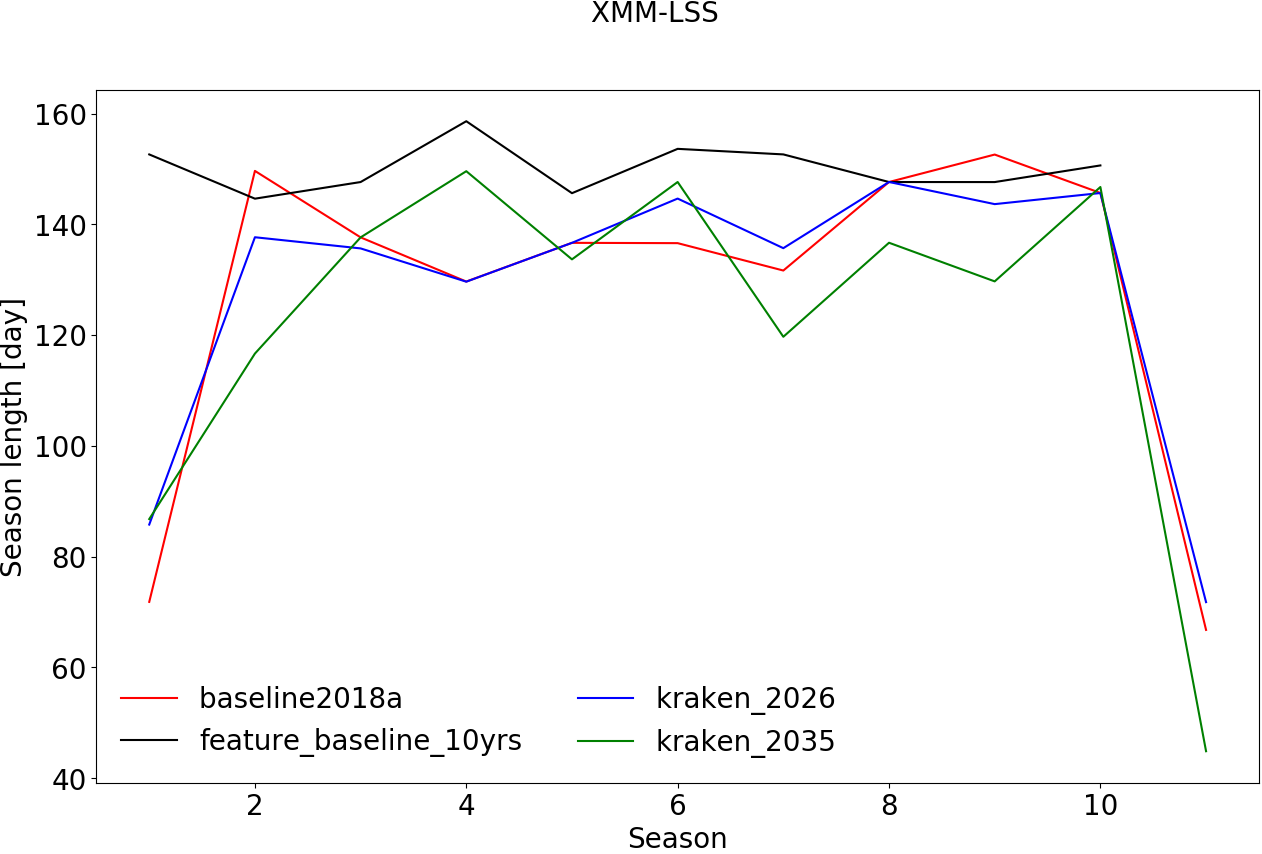
\includegraphics[width=9cm]{overview_strategy/XMM-LSS_season_length.png}
  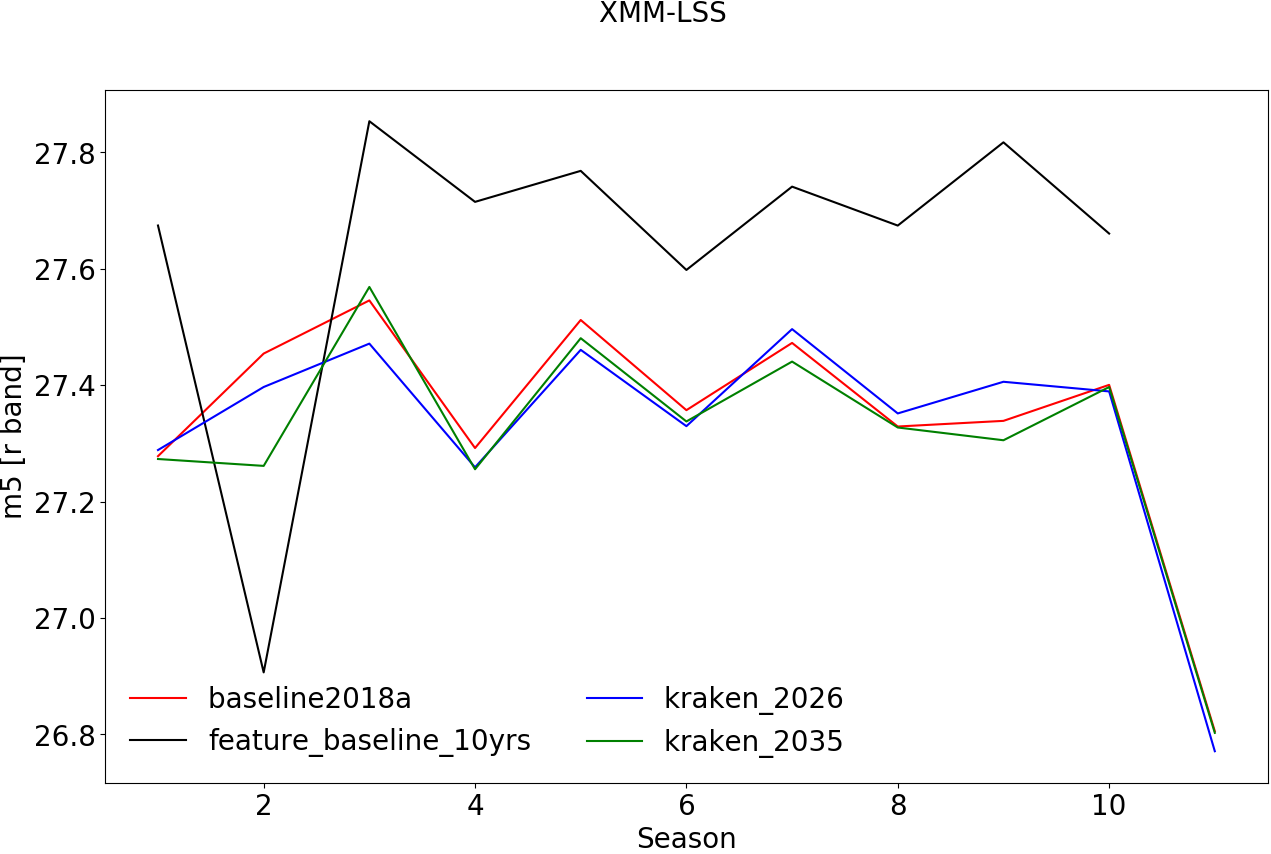
\includegraphics[width=9cm]{overview_strategy/XMM-LSS_m5.png}
  %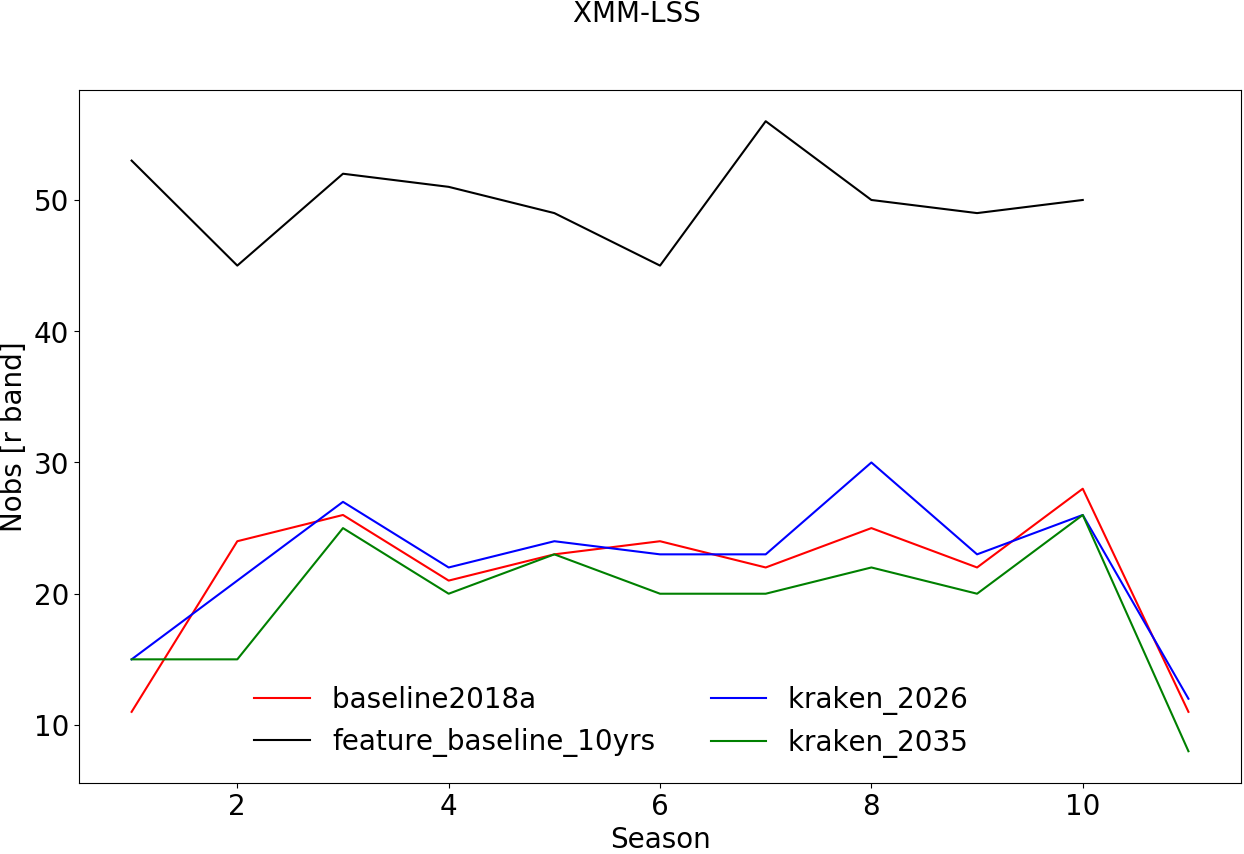
\includegraphics[width=9cm]{overview_strategy/XMM-LSS_Nobs.png}
 \caption{Cadence (top, in day), season length (middle, in day) and coadded m5 (bottom, in mag) as a function of the season for the XMM-LSS field and baseline18a, feature\_baseline\_10yrs, kralen\_2026 and kraken\_2035 observing strategies.}\label{fig:xmm-lss_cad}
\end{center}
\end{figure}

\begin{figure}[!htbp]
\begin{center}
  
  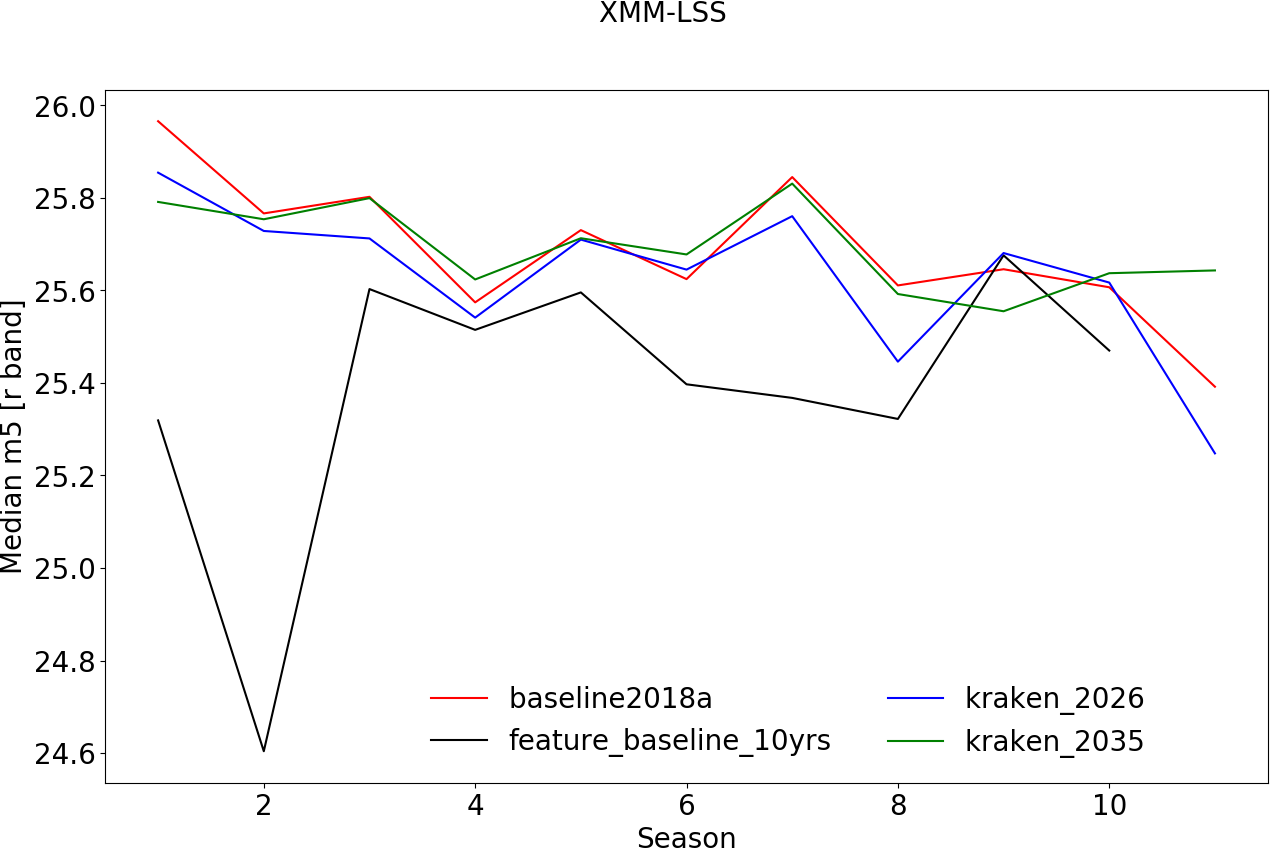
\includegraphics[width=9cm]{overview_strategy/XMM-LSS_med_m5.png}
  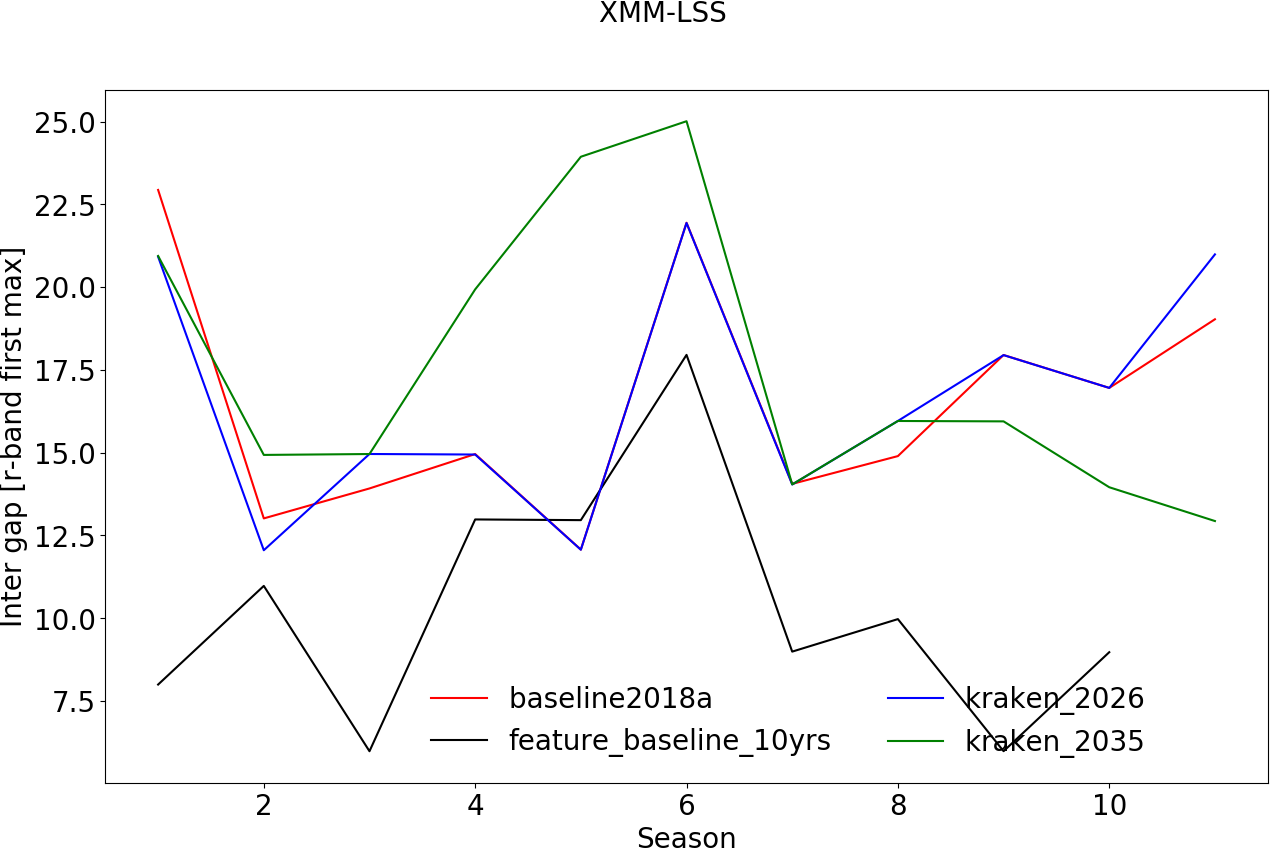
\includegraphics[width=9cm]{overview_strategy/XMM-LSS_intergap_max1.png}
    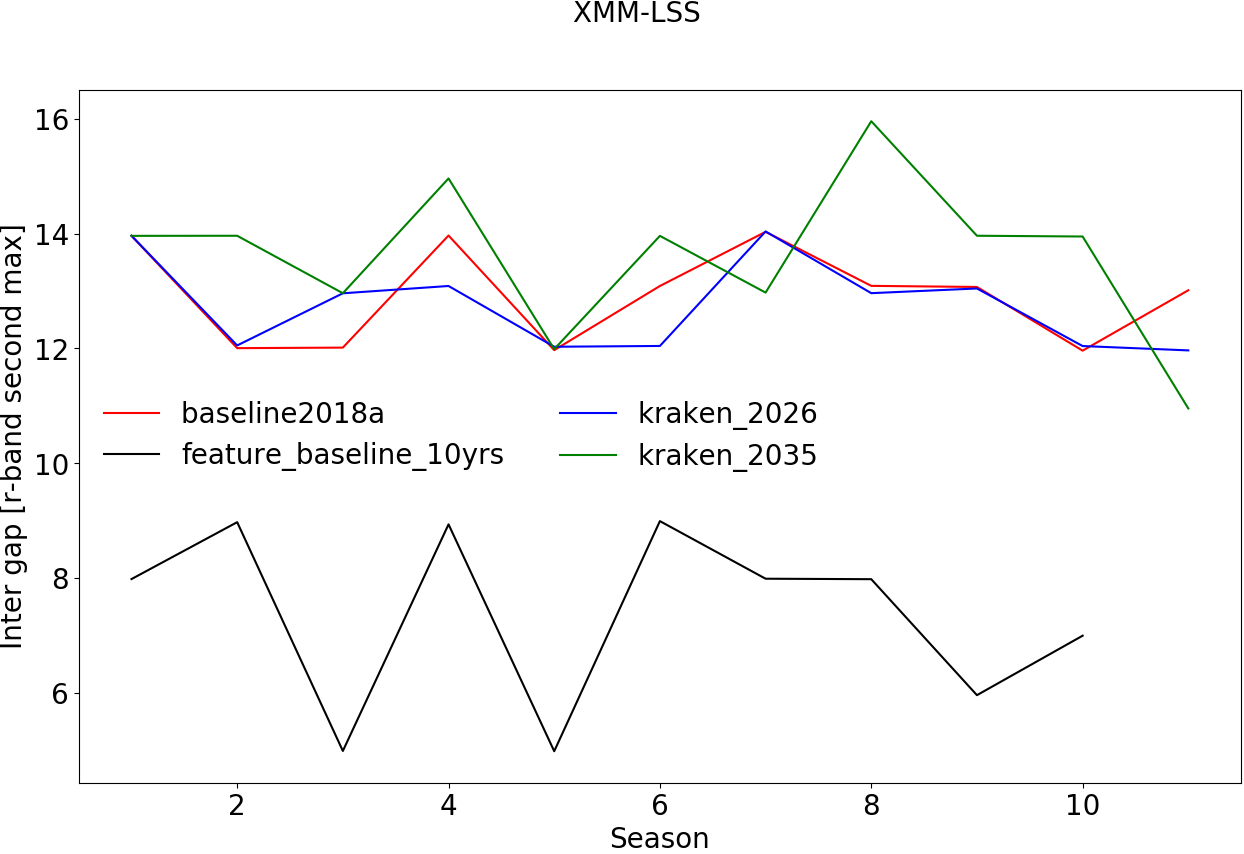
\includegraphics[width=9cm]{overview_strategy/XMM-LSS_intergap_max2.png}
 \caption{Median m5 (top, in mag), first maximum inter-night gap (middle, in day) and second maximum inter-night gap (bottom, in day)  as a function of the season for the XMM-LSS field and baseline18a, feature\_baseline\_10yrs, kralen\_2026 and kraken\_2035 observing strategies.}\label{fig:xmm-lss_m5}
\end{center}
\end{figure}


%%%%%%%%%%%%%%%%%%%%%%%%%%%%%%%%%%%%%%%%%%%%%%


\begin{figure}[!htbp]
\begin{center}
  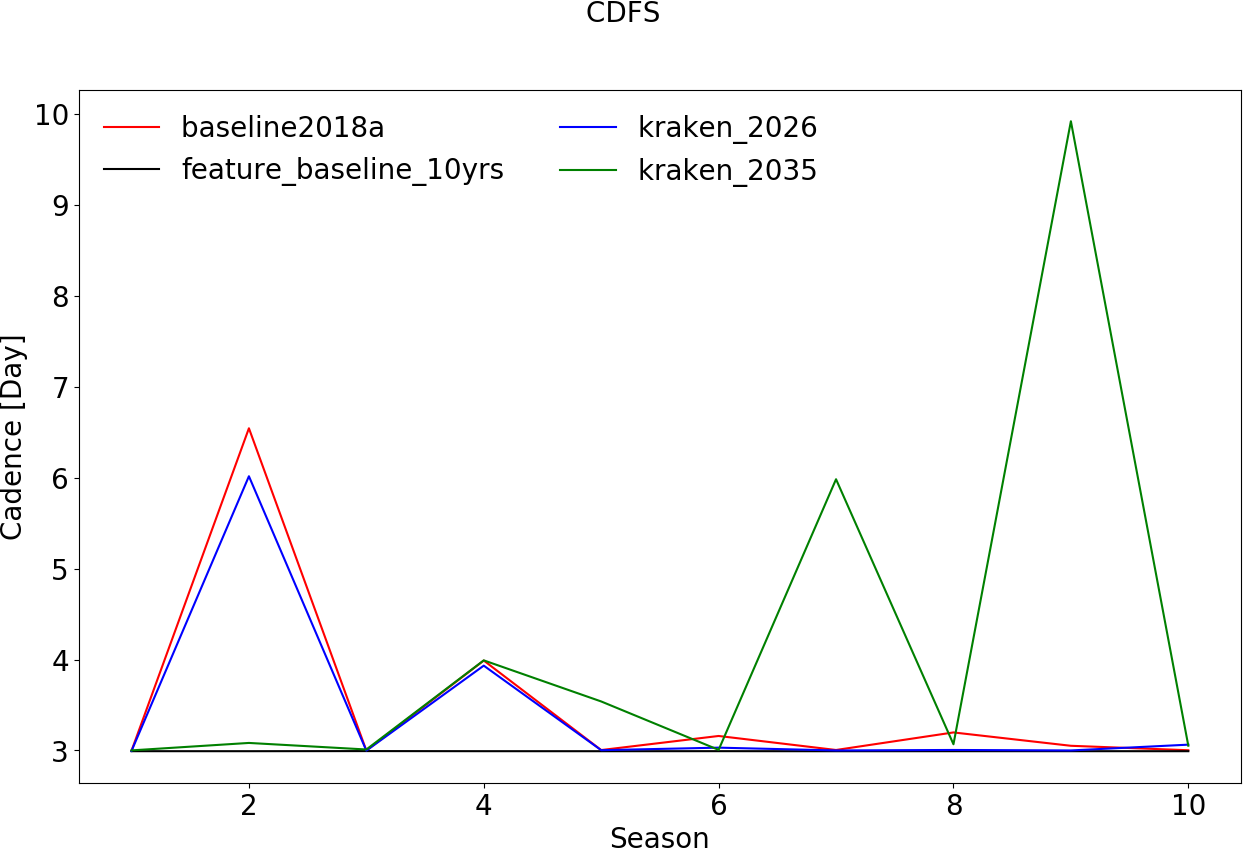
\includegraphics[width=9cm]{overview_strategy/CDFS_cadence.png}
  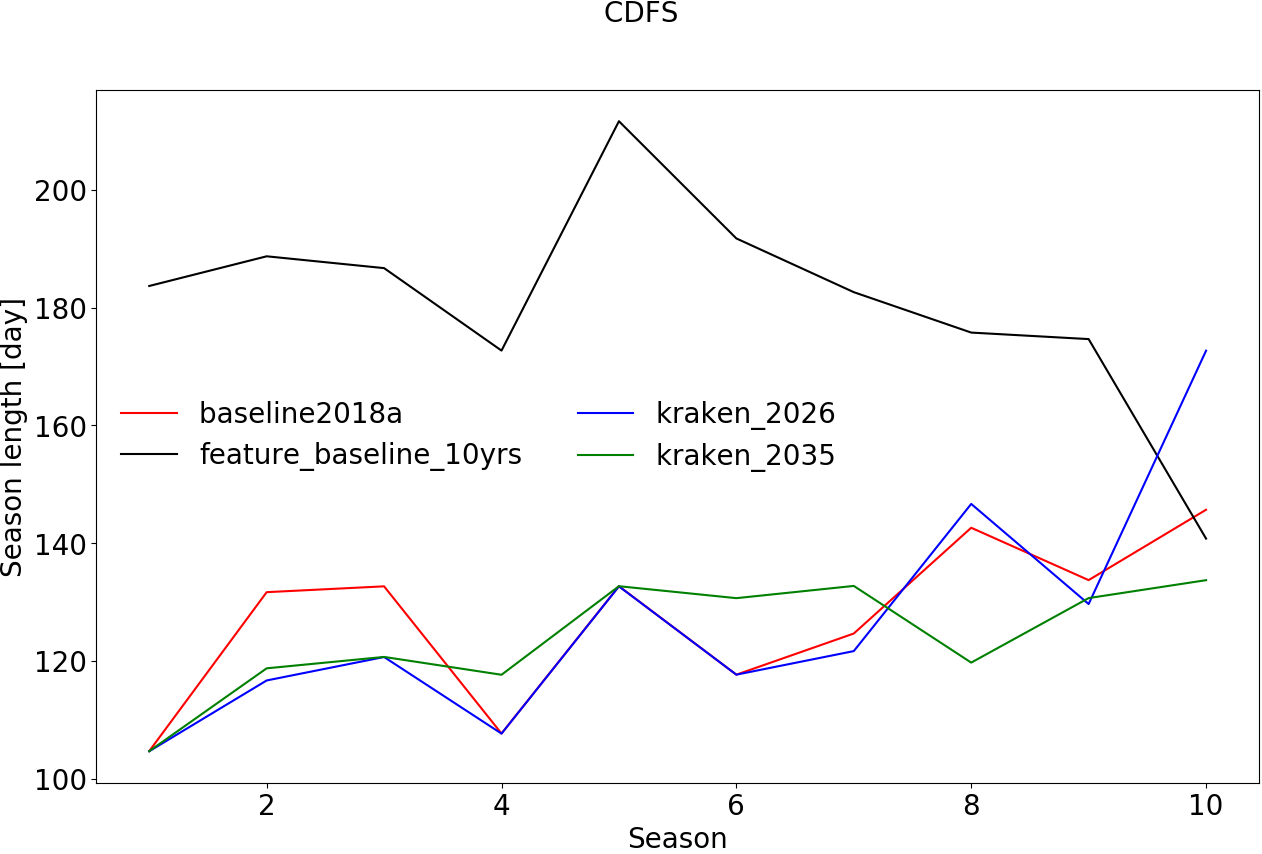
\includegraphics[width=9cm]{overview_strategy/CDFS_season_length.png}
  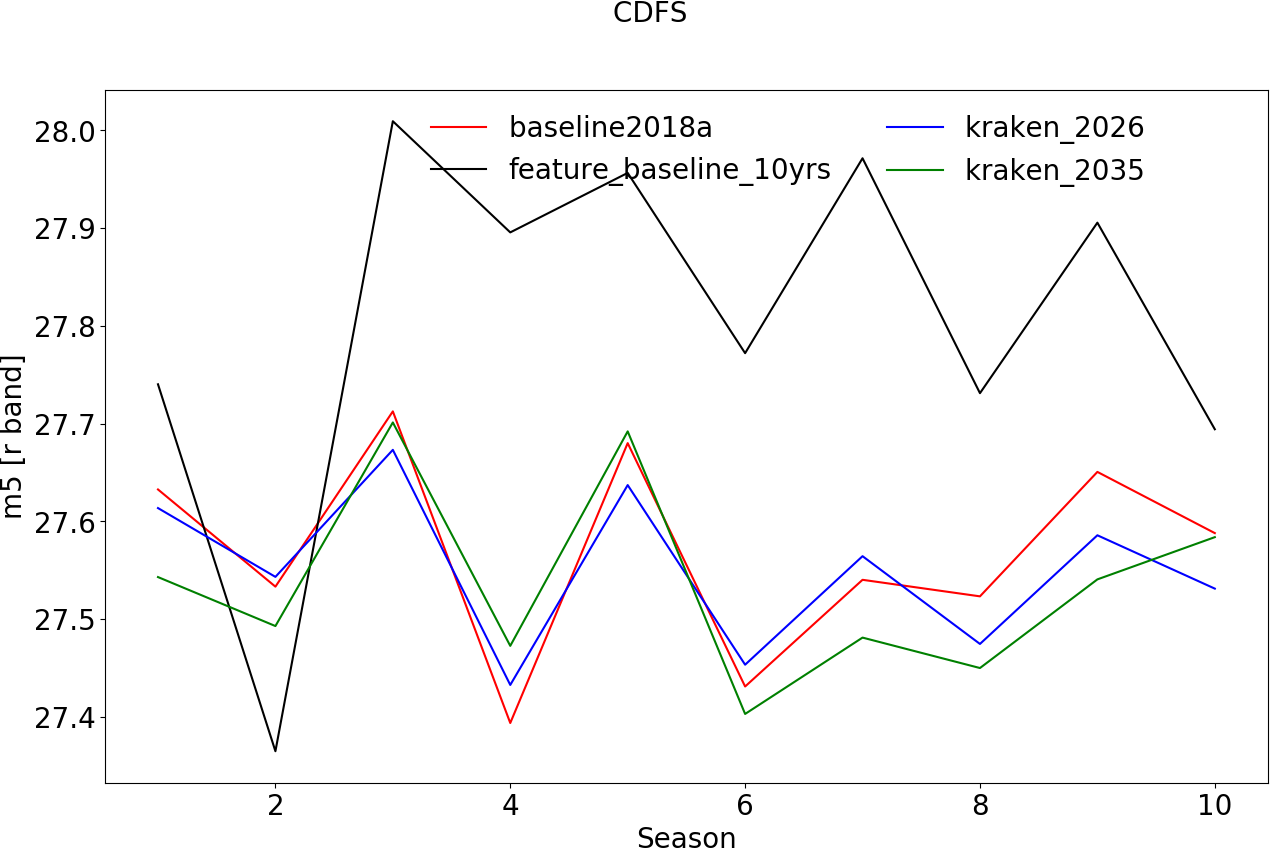
\includegraphics[width=9cm]{overview_strategy/CDFS_m5.png}
  %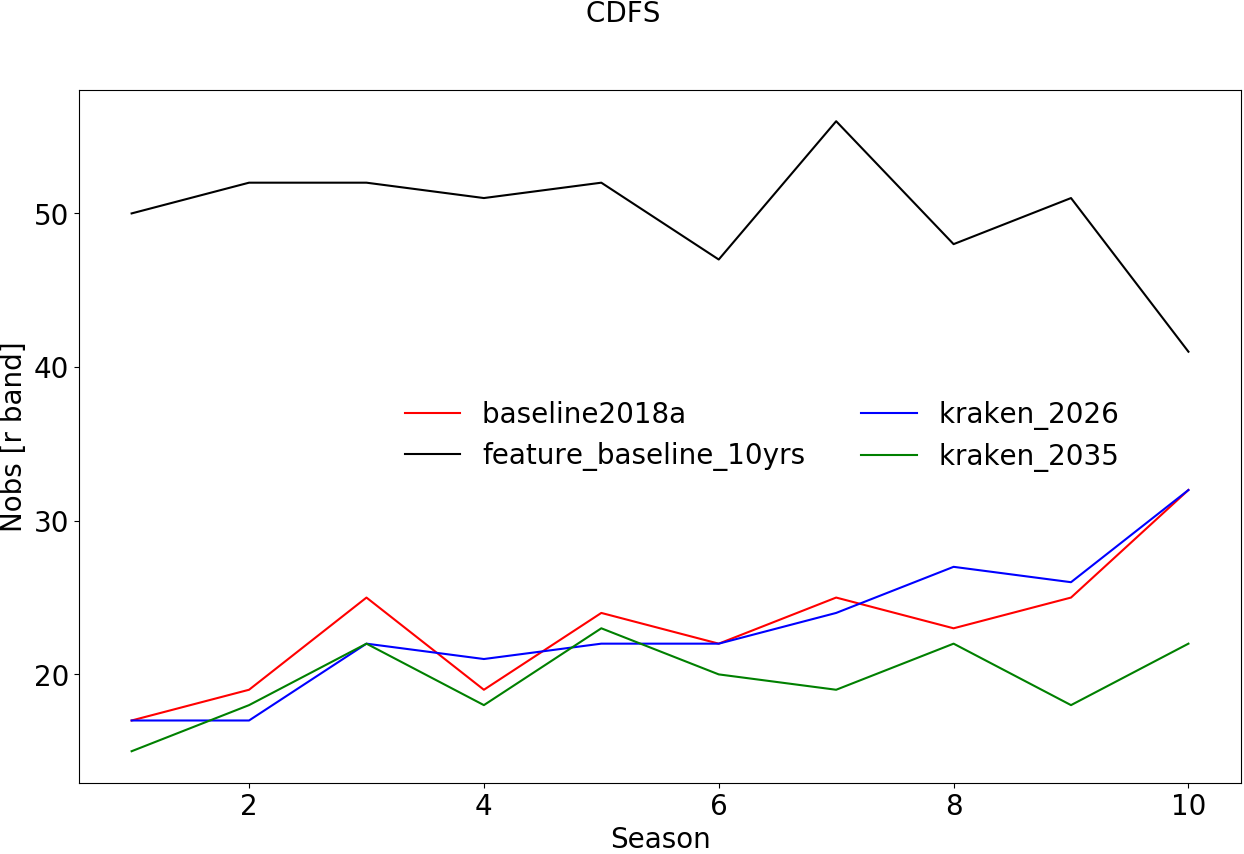
\includegraphics[width=9cm]{overview_strategy/CDFS_Nobs.png}
 \caption{Cadence (top, in day), season length (middle, in day) and coadded m5 (bottom, in mag) as a function of the season for the CDFS field and baseline18a, feature\_baseline\_10yrs, kralen\_2026 and kraken\_2035 observing strategies.}\label{fig:cdfs_cad}
\end{center}
\end{figure}

\begin{figure}[!htbp]
\begin{center}
  
  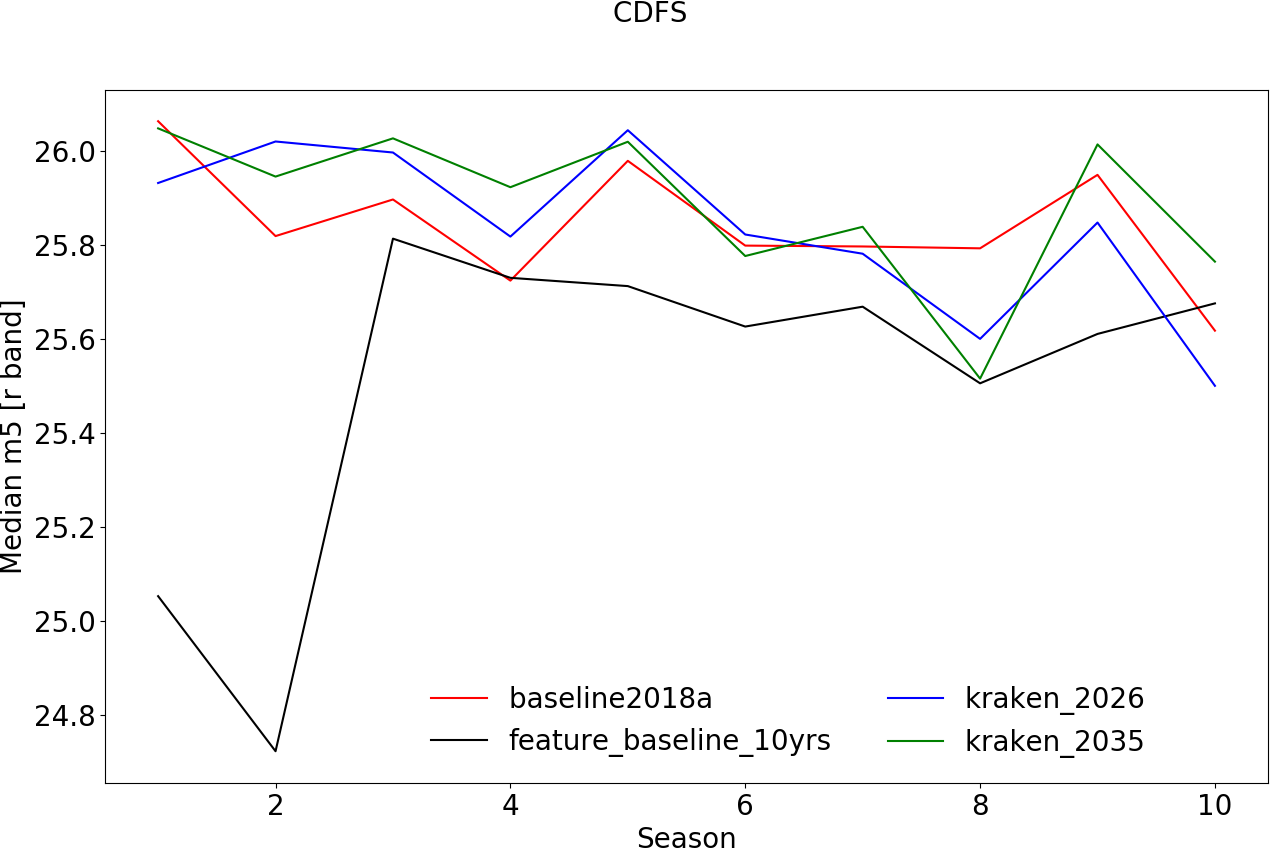
\includegraphics[width=9cm]{overview_strategy/CDFS_med_m5.png}
  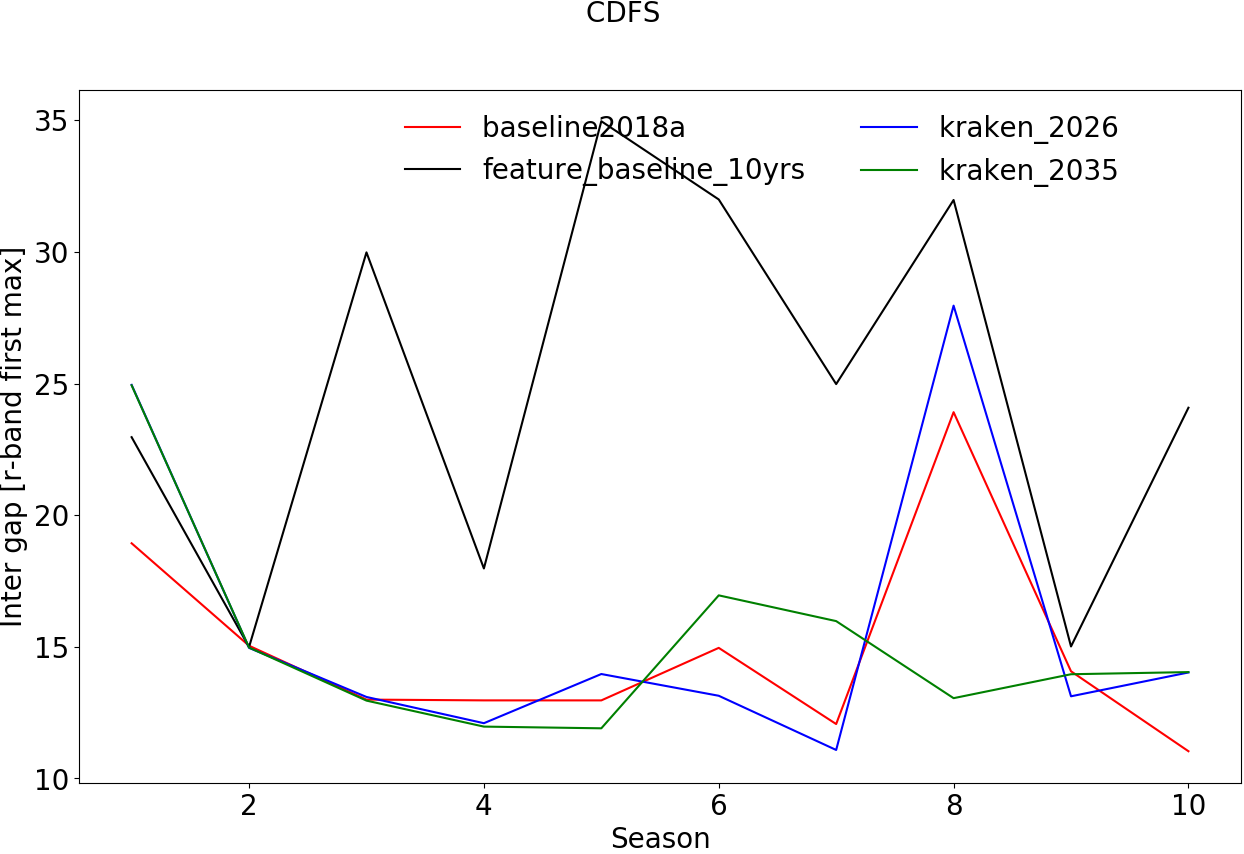
\includegraphics[width=9cm]{overview_strategy/CDFS_intergap_max1.png}
    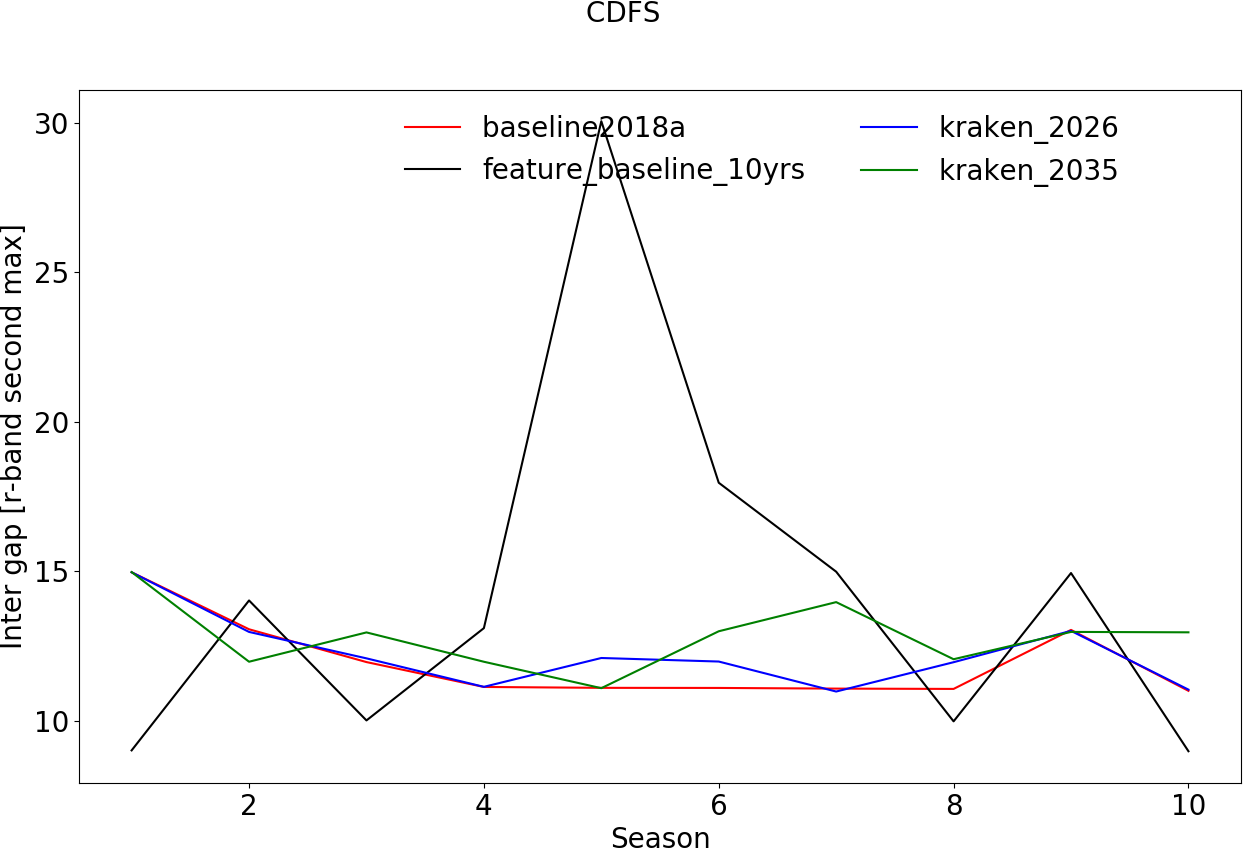
\includegraphics[width=9cm]{overview_strategy/CDFS_intergap_max2.png}
 \caption{Median m5 (top, in mag), first maximum inter-night gap (middle, in day) and second maximum inter-night gap (bottom, in day)  as a function of the season for the CDFS field and baseline18a, feature\_baseline\_10yrs, kralen\_2026 and kraken\_2035 observing strategies.}\label{fig:cdfs_m5}
\end{center}
\end{figure}


%%%%%%%%%%%%%%%%%%%%%%%%%%%%%%%%%%%%%%%%%%%%%%


\begin{figure}[!htbp]
\begin{center}
  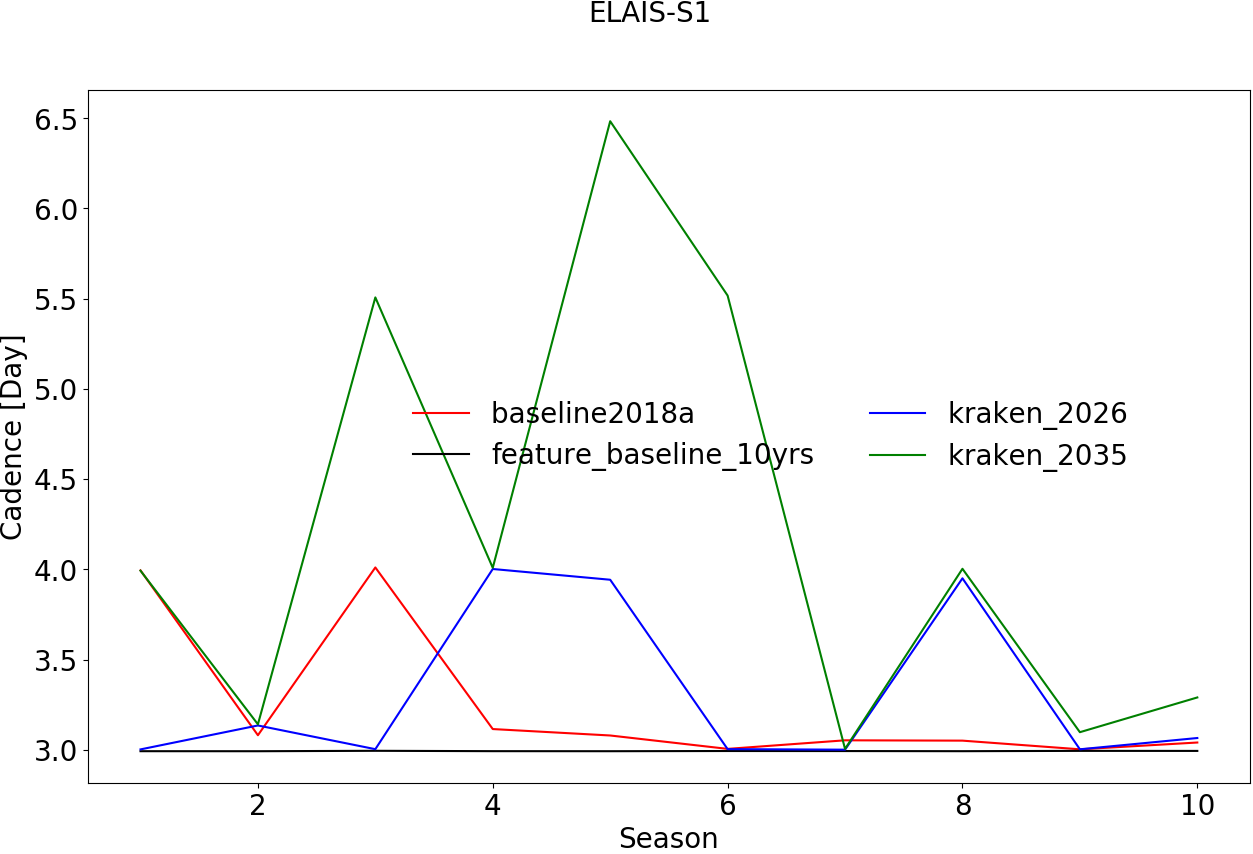
\includegraphics[width=9cm]{overview_strategy/ELAIS-S1_cadence.png}
  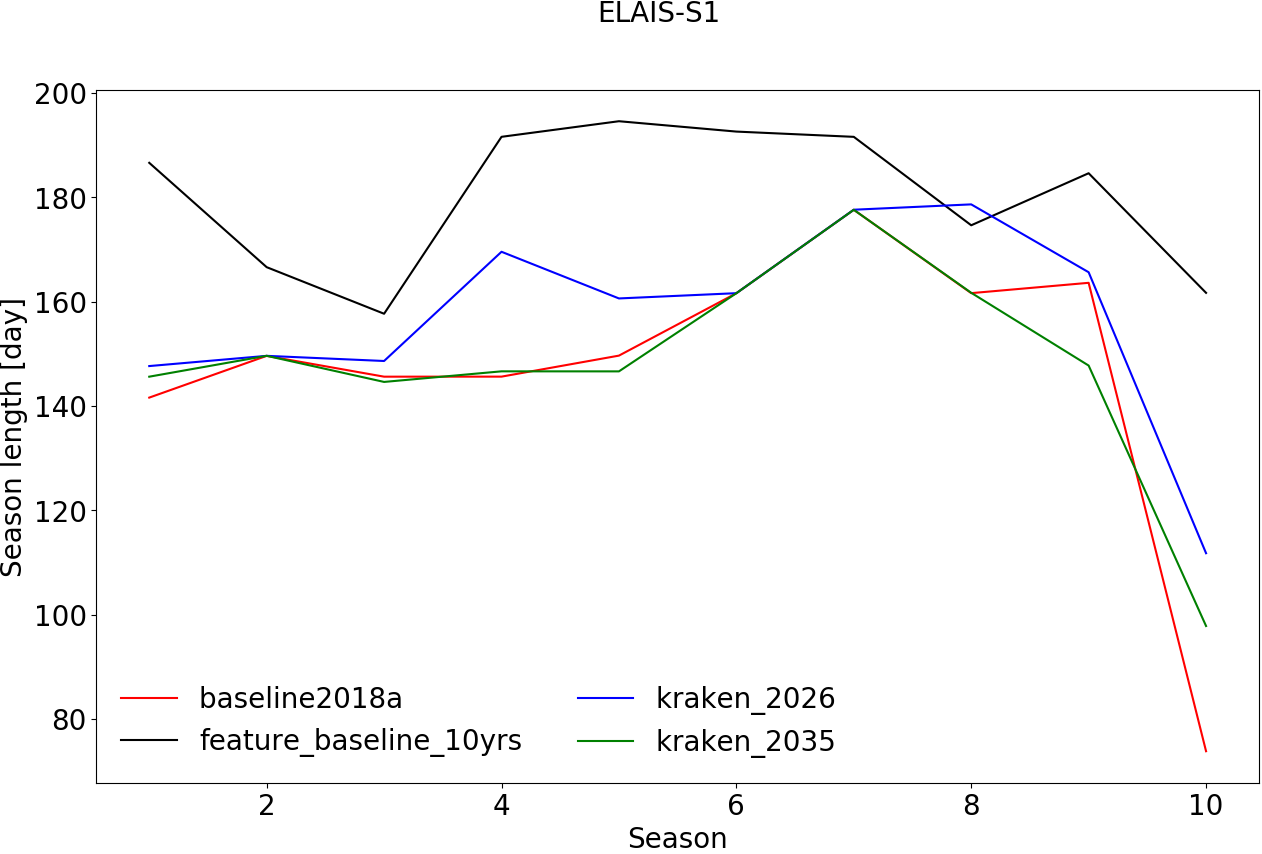
\includegraphics[width=9cm]{overview_strategy/ELAIS-S1_season_length.png}
  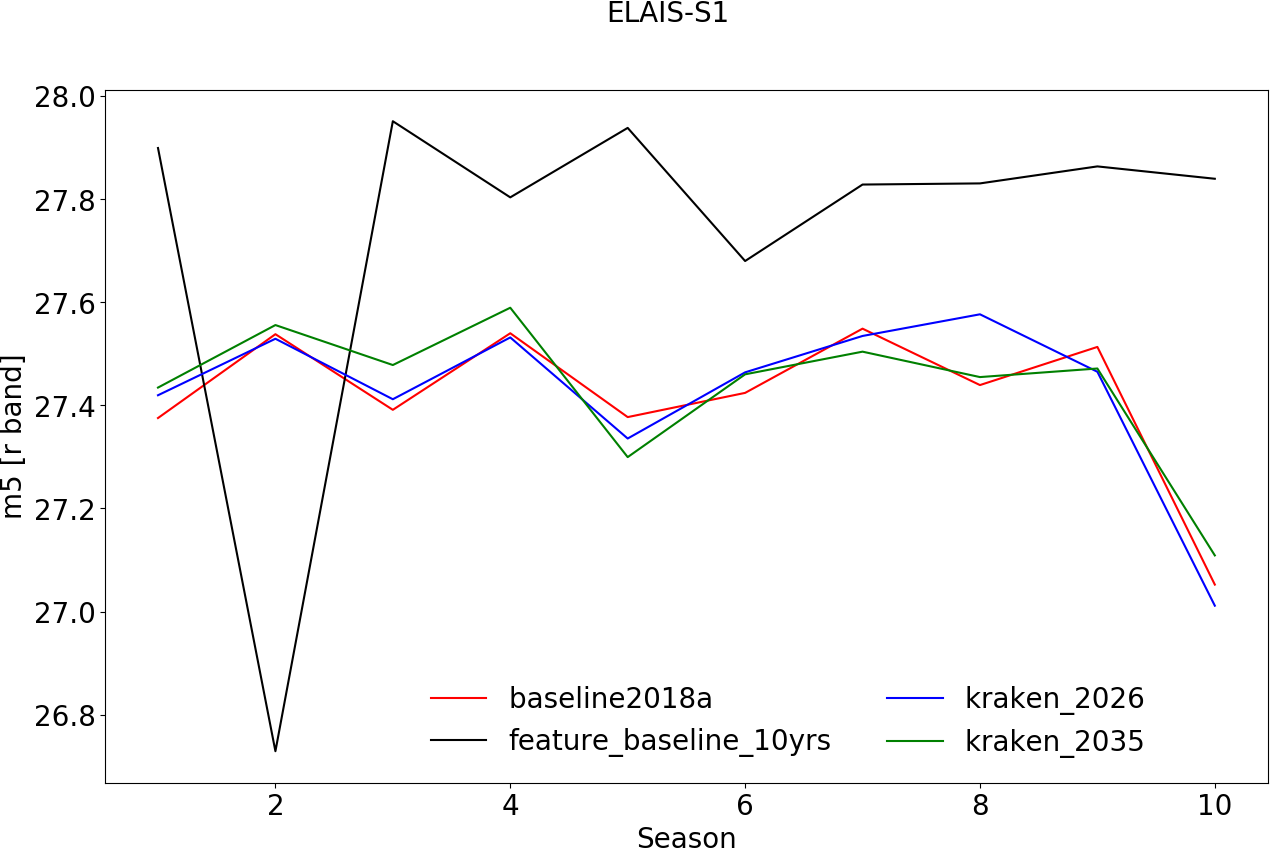
\includegraphics[width=9cm]{overview_strategy/ELAIS-S1_m5.png}
  %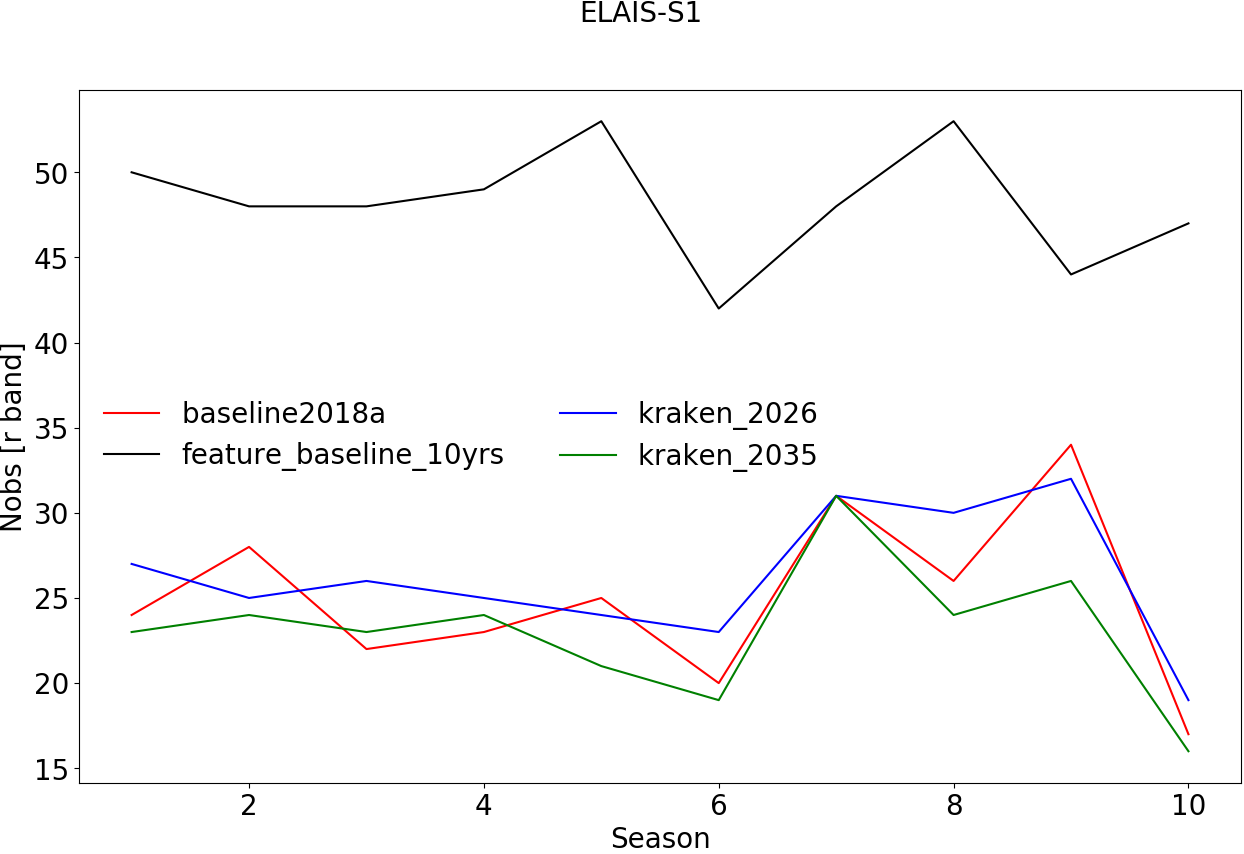
\includegraphics[width=9cm]{overview_strategy/ELAIS-S1_Nobs.png}
 \caption{Cadence (top, in day), season length (middle, in day) and coadded m5 (bottom, in mag) as a function of the season for the ELAIS-S1 field and baseline18a, feature\_baseline\_10yrs, kralen\_2026 and kraken\_2035 observing strategies.}\label{fig:elais-s1_cad}
\end{center}
\end{figure}

\begin{figure}[!htbp]
\begin{center}
  
  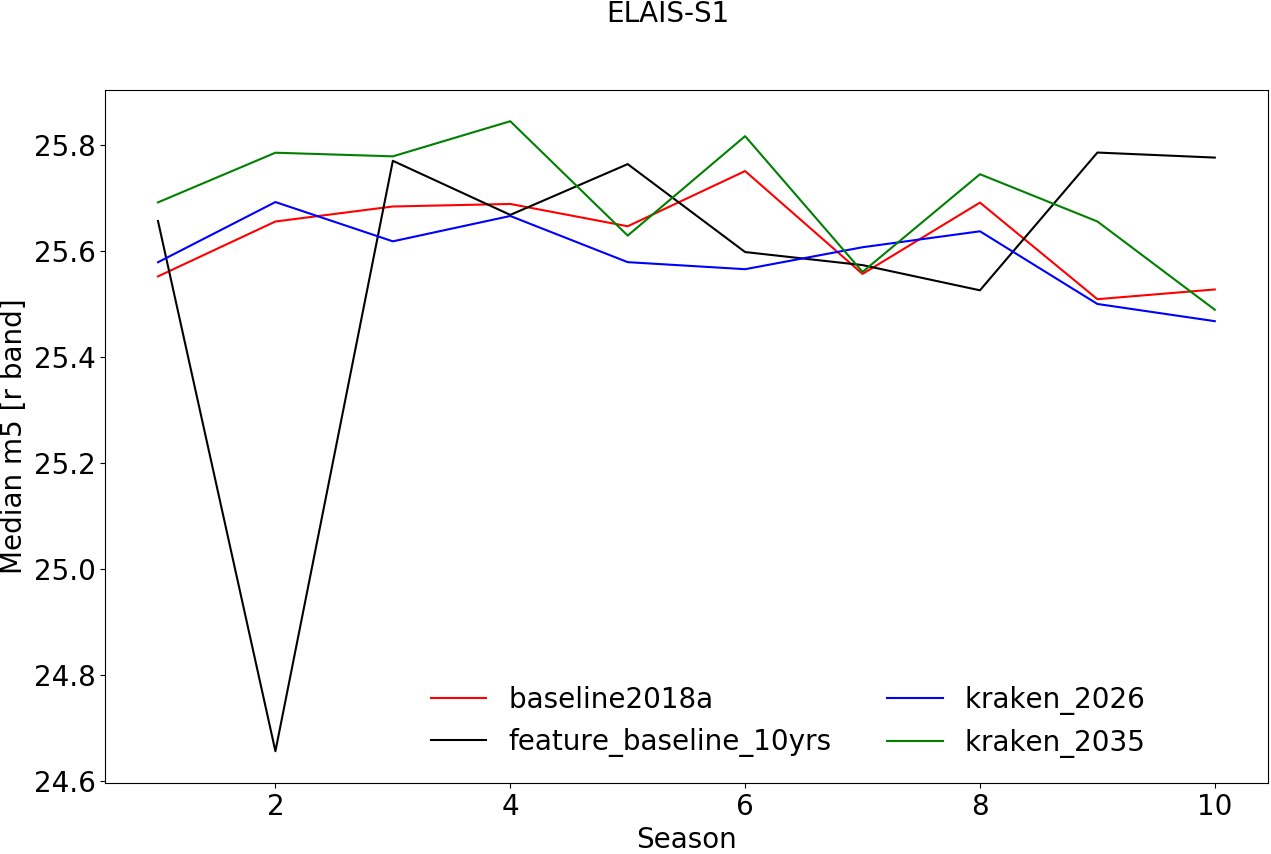
\includegraphics[width=9cm]{overview_strategy/ELAIS-S1_med_m5.png}
  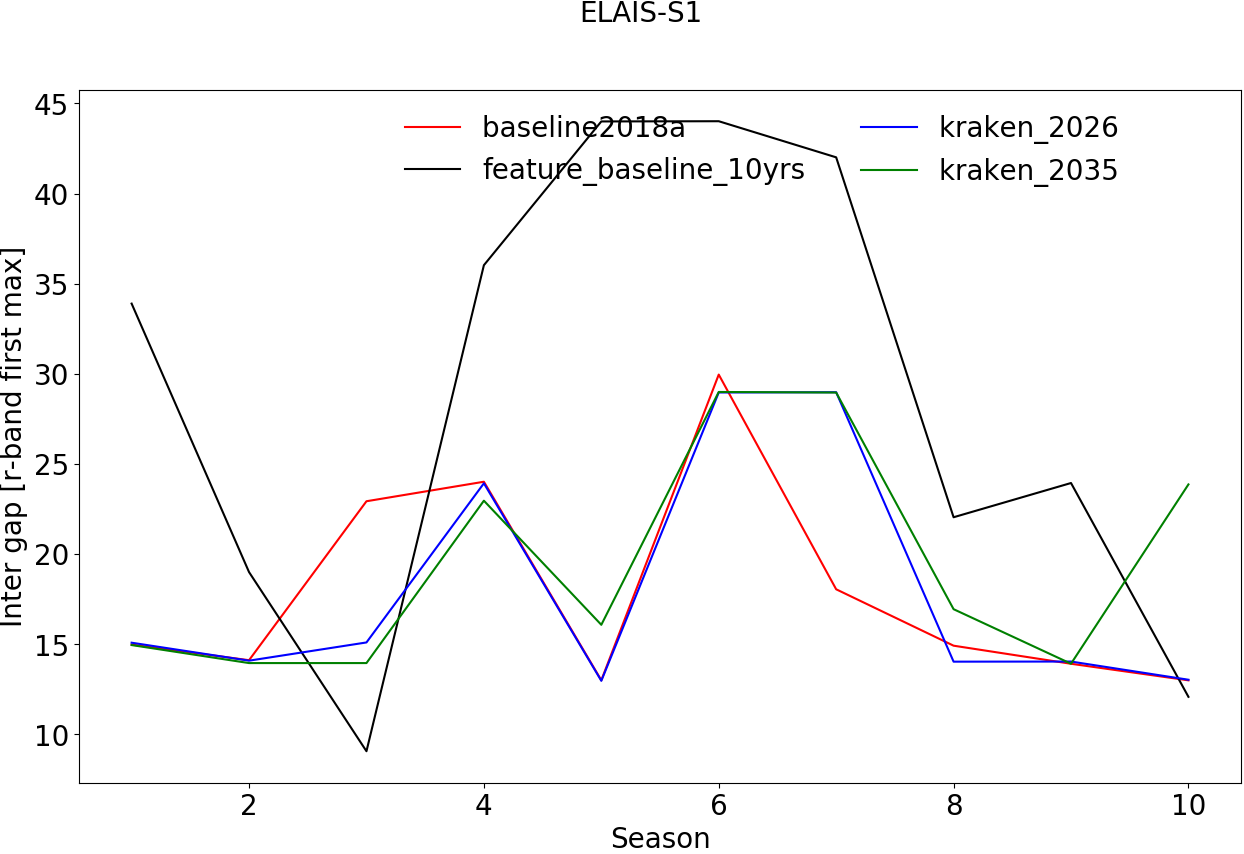
\includegraphics[width=9cm]{overview_strategy/ELAIS-S1_intergap_max1.png}
    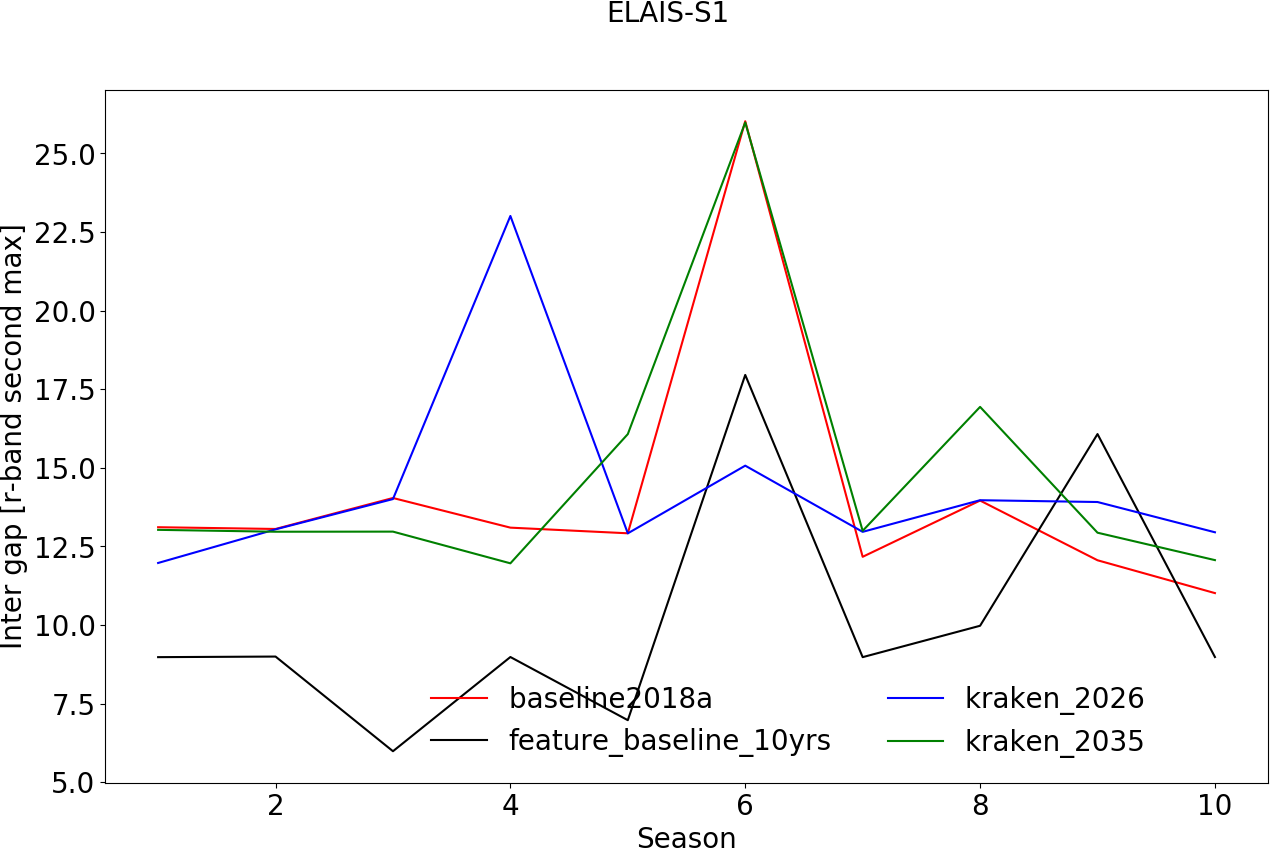
\includegraphics[width=9cm]{overview_strategy/ELAIS-S1_intergap_max2.png}
 \caption{Median m5 (top, in mag), first maximum inter-night gap (middle, in day) and second maximum inter-night gap (bottom, in day)  as a function of the season for the ELAIS-S1 field and baseline18a, feature\_baseline\_10yrs, kralen\_2026 and kraken\_2035 observing strategies.}\label{fig:elais-s1_m5}
\end{center}
\end{figure}


%%%%%%%%%%%%%%%%%%%%%%%%%%%%%%%%%%%%%%%%%%%%%%


\begin{figure}[!htbp]
\begin{center}
  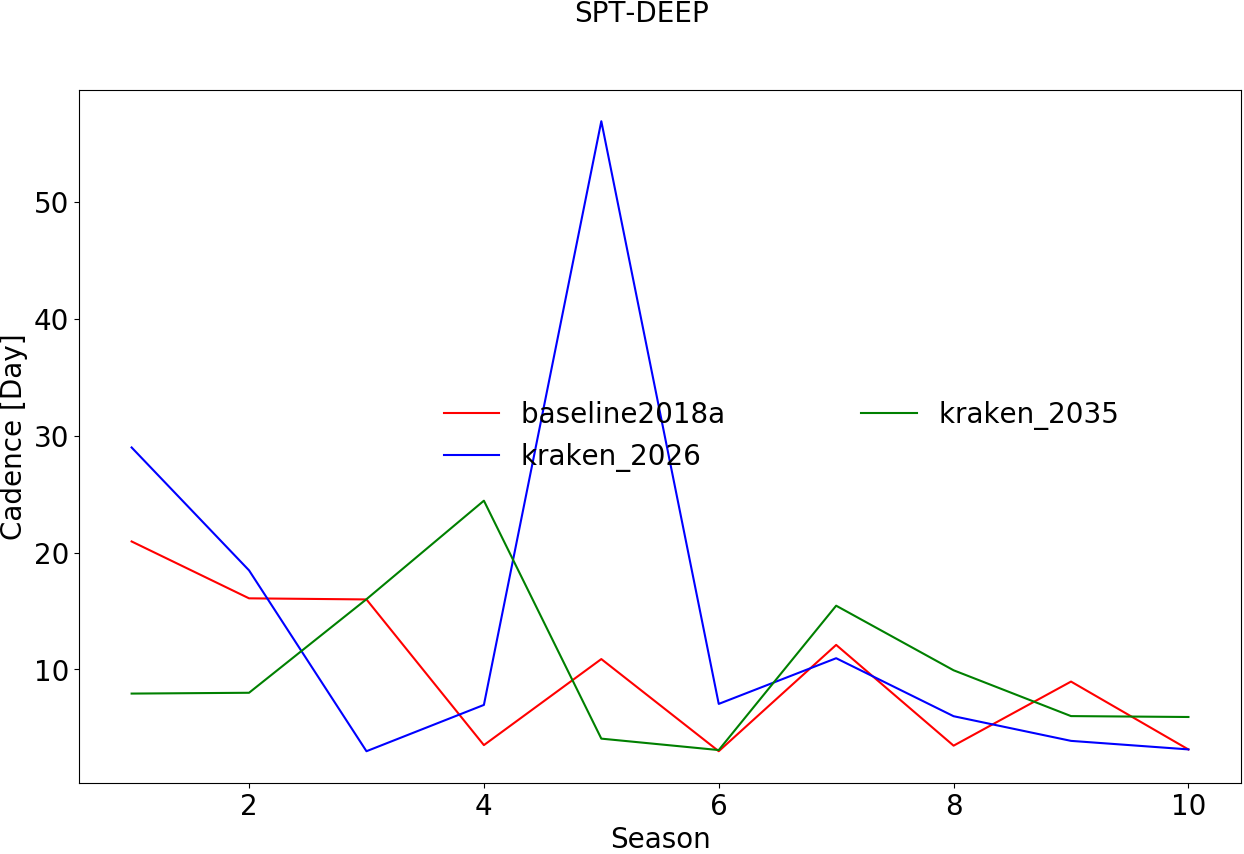
\includegraphics[width=9cm]{overview_strategy/SPT-DEEP_cadence.png}
  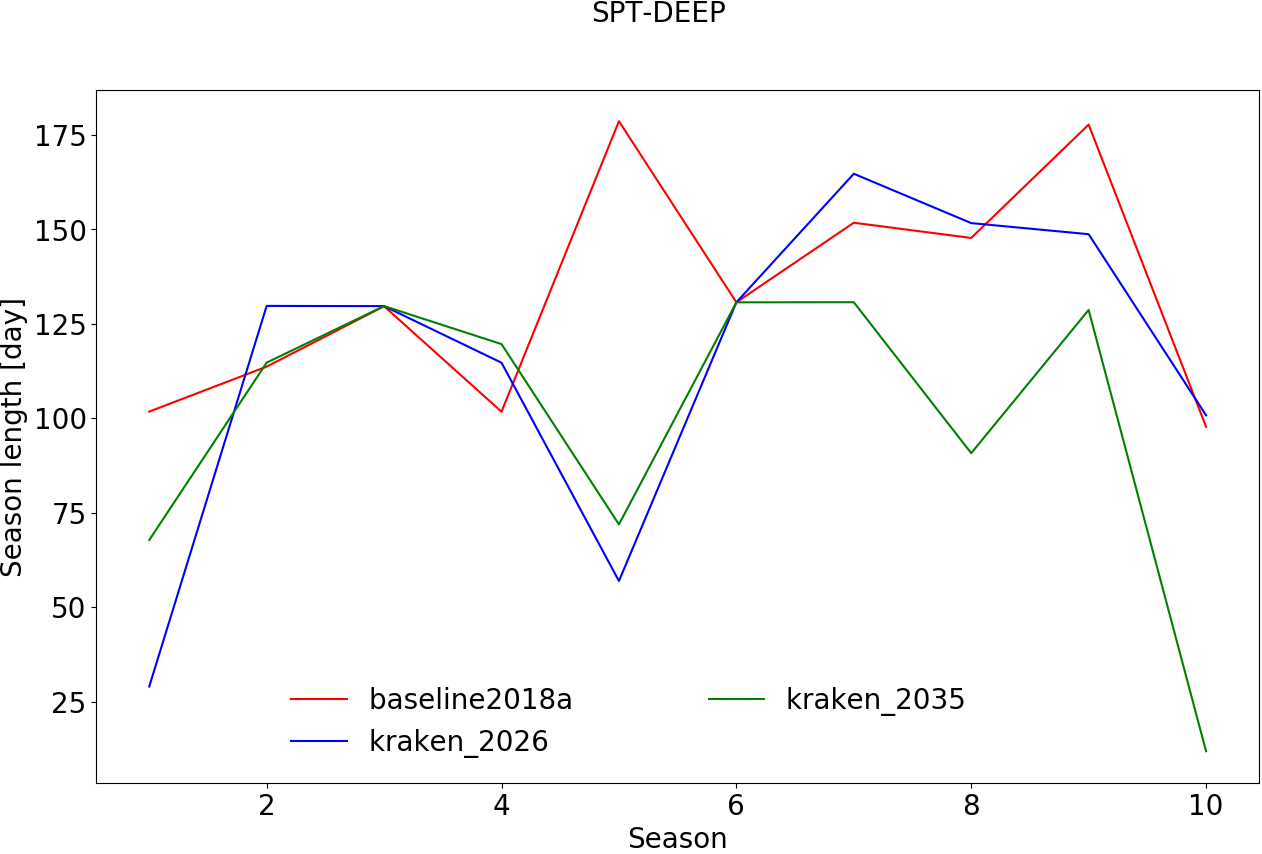
\includegraphics[width=9cm]{overview_strategy/SPT-DEEP_season_length.png}
  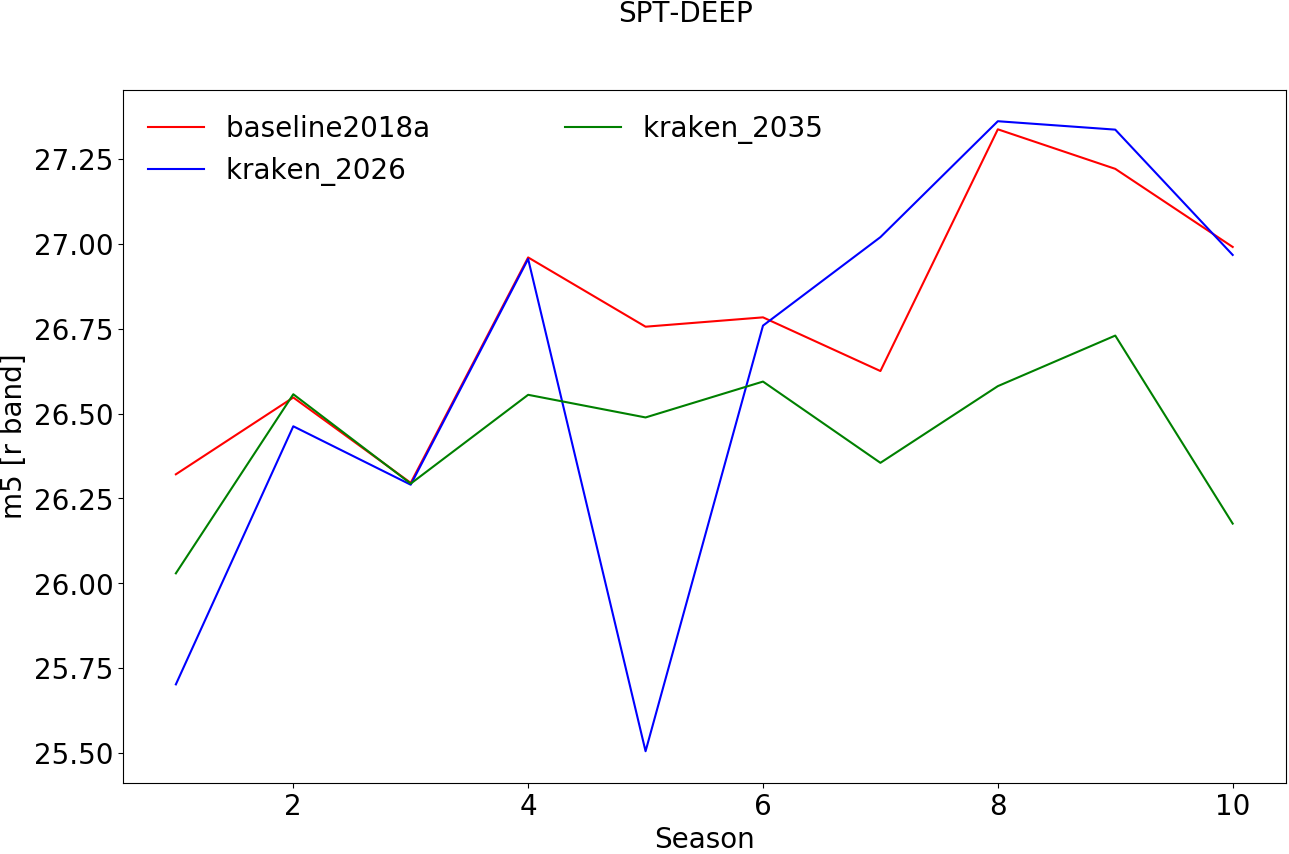
\includegraphics[width=9cm]{overview_strategy/SPT-DEEP_m5.png}
  %\includegraphics[width=9cm]{overview_strategy/SPT DEEP_Nobs.png}
 \caption{Cadence (top, in day), season length (middle, in day) and coadded m5 (bottom, in mag) as a function of the season for the SPT DEEP field and baseline18a, feature\_baseline\_10yrs, kralen\_2026 and kraken\_2035 observing strategies.}\label{fig:spt deep_cad}
\end{center}
\end{figure}

\begin{figure}[!htbp]
\begin{center}
  
  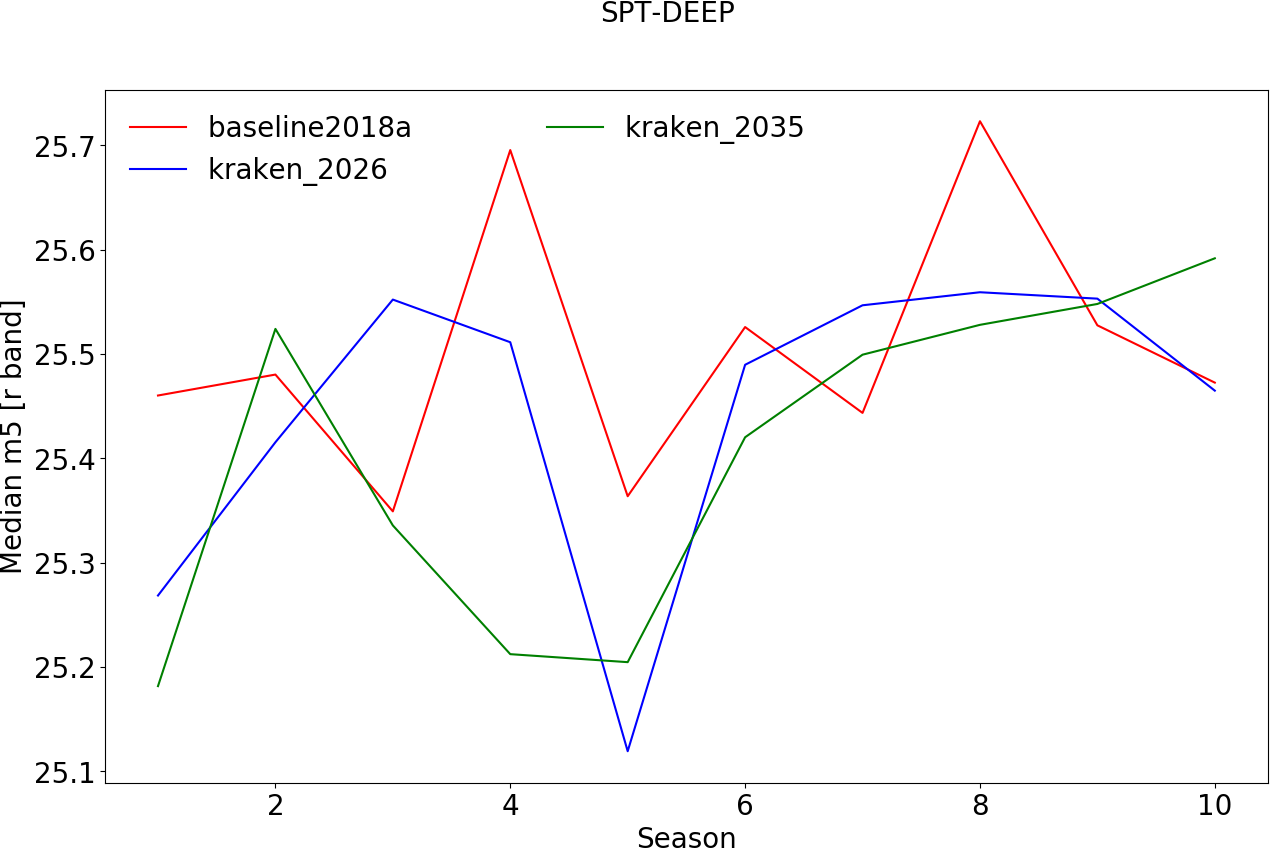
\includegraphics[width=9cm]{overview_strategy/SPT-DEEP_med_m5.png}
  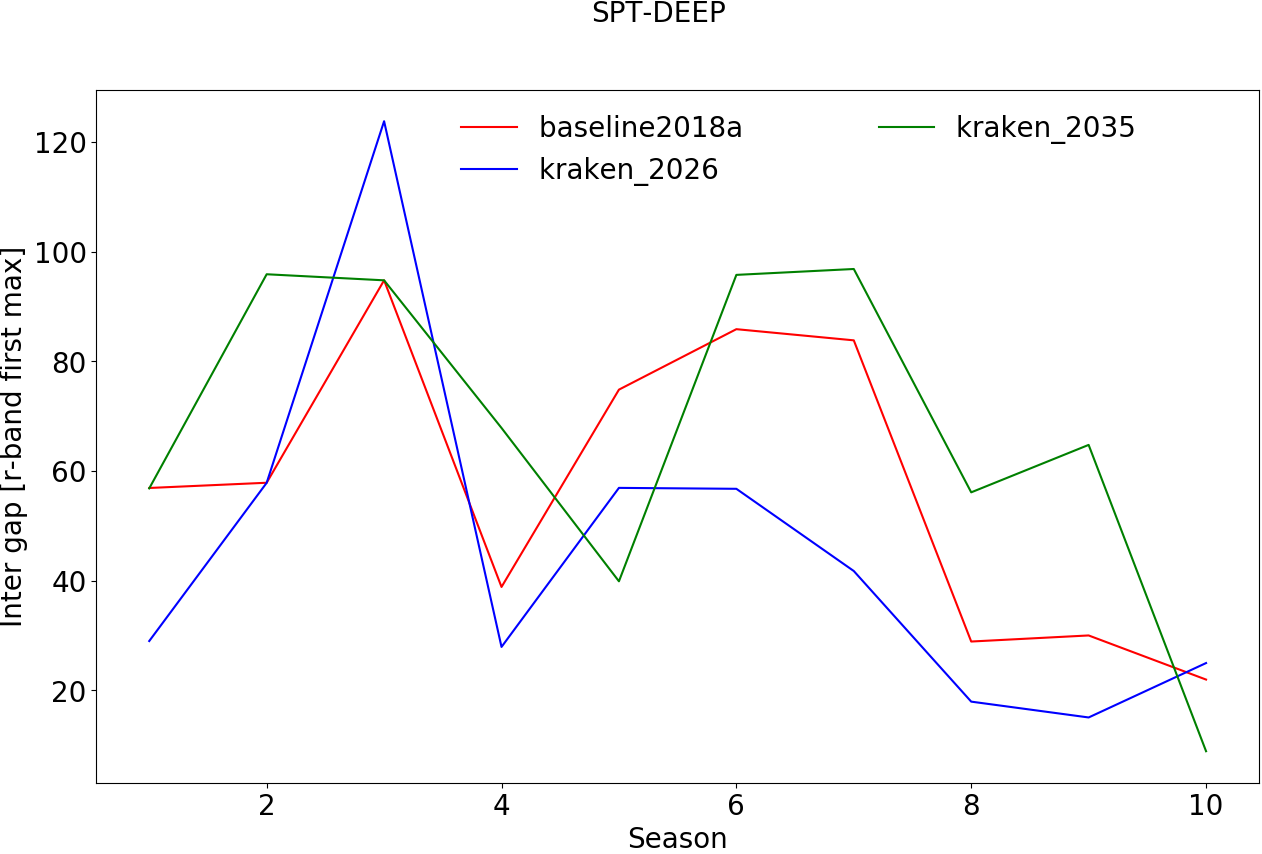
\includegraphics[width=9cm]{overview_strategy/SPT-DEEP_intergap_max1.png}
    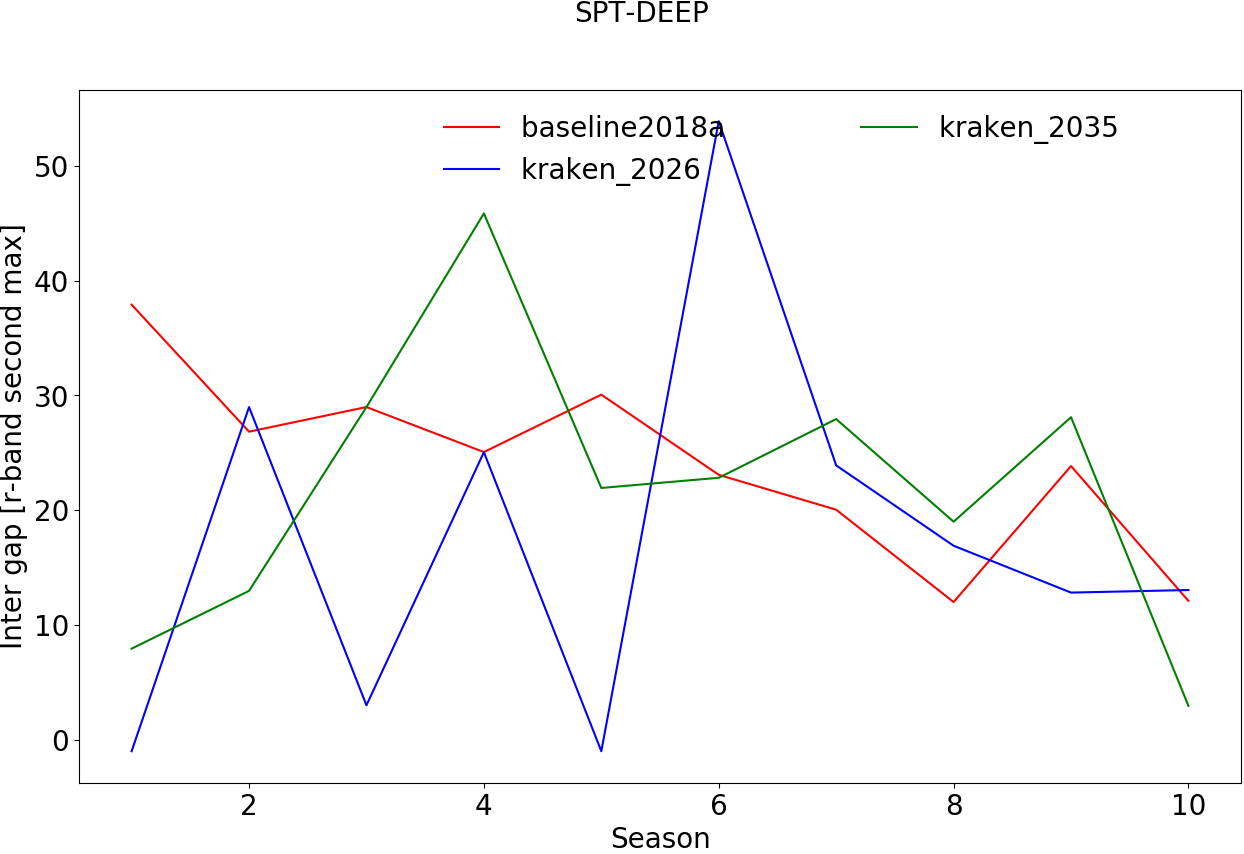
\includegraphics[width=9cm]{overview_strategy/SPT-DEEP_intergap_max2.png}
 \caption{Median m5 (top, in mag), first maximum inter-night gap (middle, in day) and second maximum inter-night gap (bottom, in day)  as a function of the season for the SPT DEEP field and baseline18a, feature\_baseline\_10yrs, kralen\_2026 and kraken\_2035 observing strategies.}\label{fig:spt deep_m5}
\end{center}
\end{figure}


%%%%%%%%%%%%%%%%%%%%%%%%%%%%%%%%%%%%%%%%%%%%%%


\begin{figure}[!htbp]
\begin{center}
  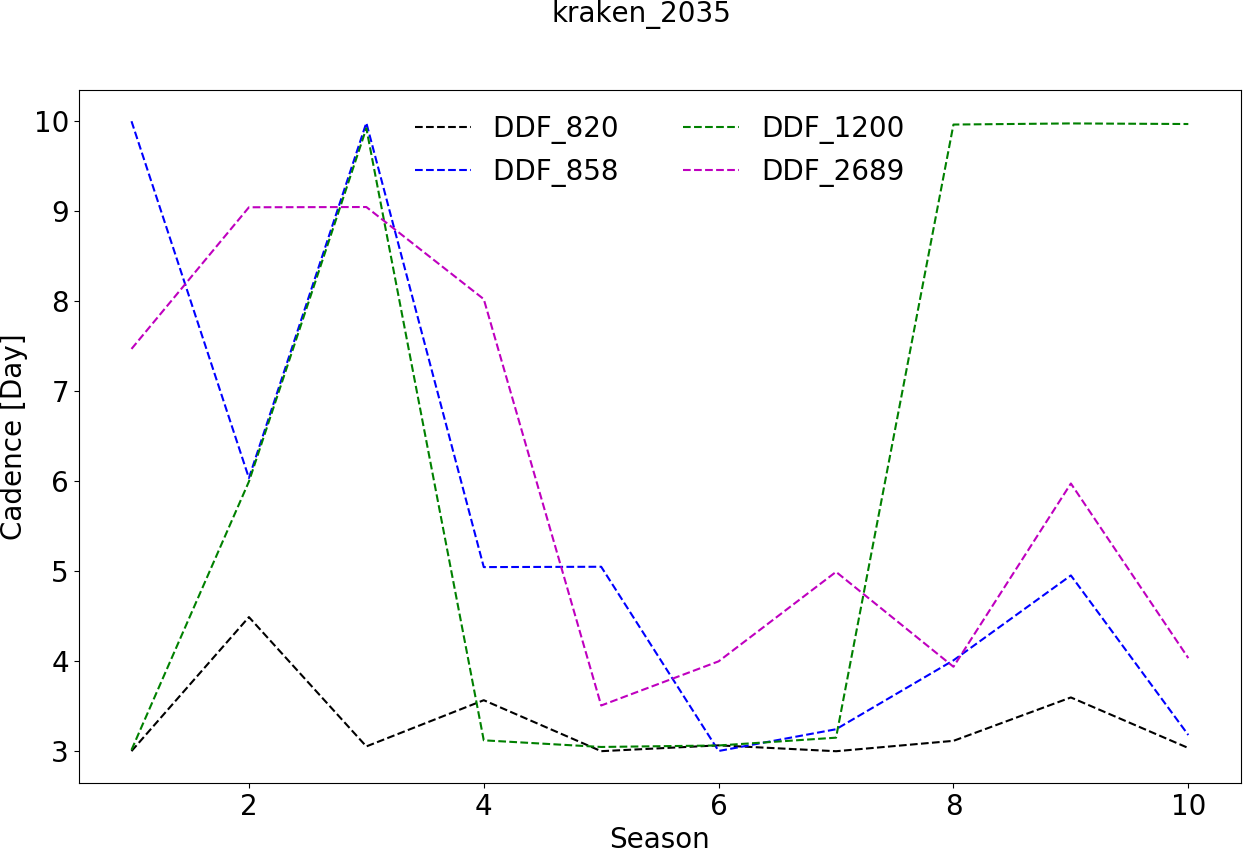
\includegraphics[width=9cm]{overview_strategy/kraken_2035_cadence.png}
  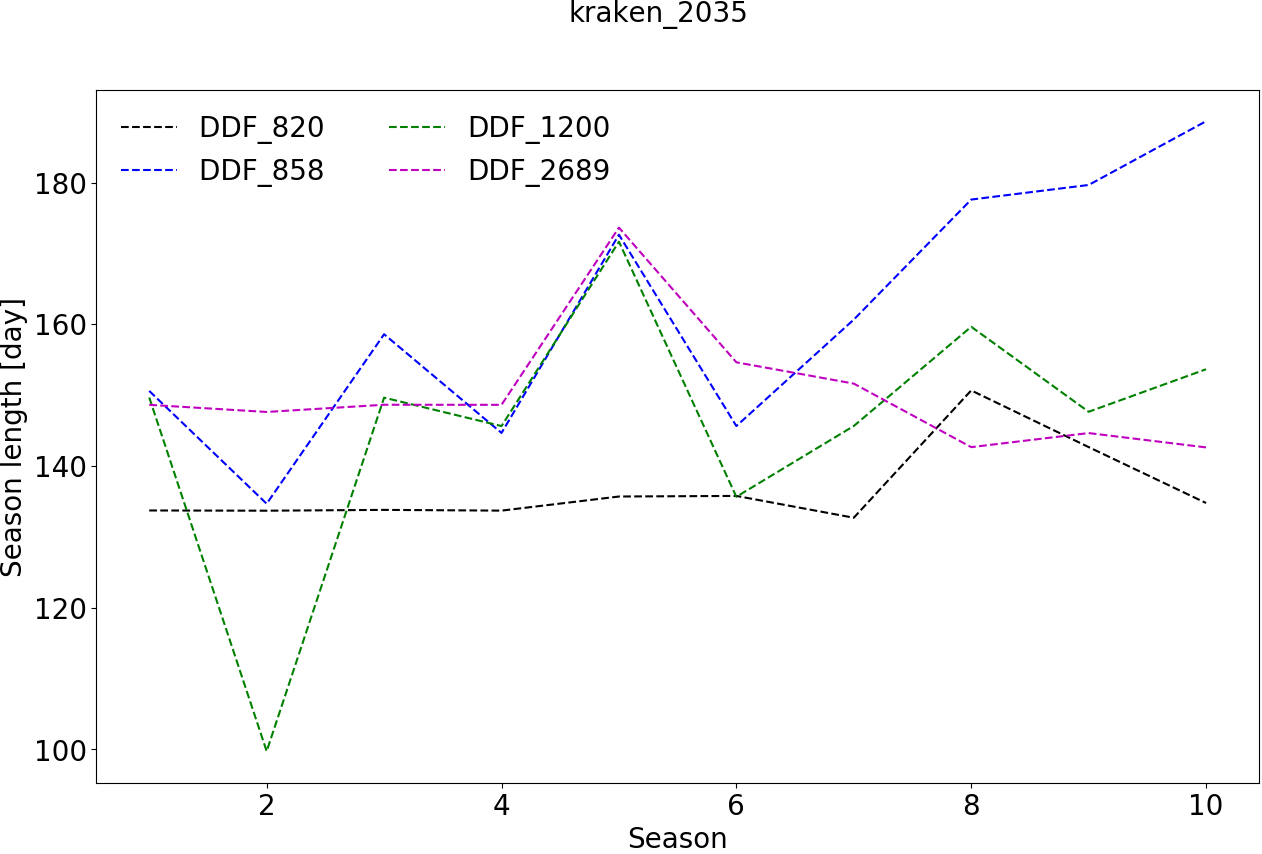
\includegraphics[width=9cm]{overview_strategy/kraken_2035_season_length.png}
  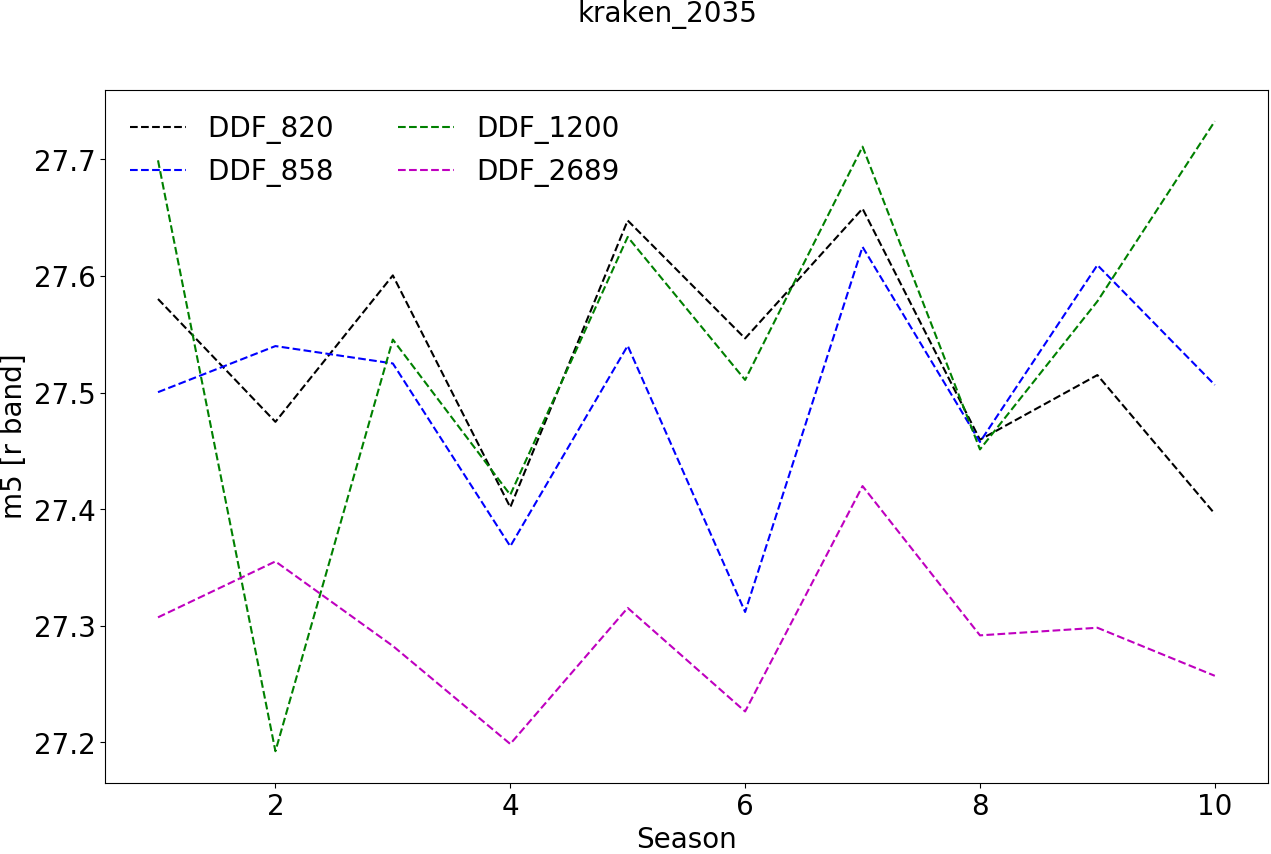
\includegraphics[width=9cm]{overview_strategy/kraken_2035_m5.png}
  %\includegraphics[width=9cm]{overview_strategy/SPT DEEP_Nobs.png}
 \caption{Cadence (top, in day), season length (middle, in day) and coadded m5 (bottom, in mag) as a function of the season for \ddfa, \ddfb, \ddfb and \ddfd fields and kraken\_2035 observing strategy.}\label{fig:kraken_cad}
\end{center}
\end{figure}

\begin{figure}[!htbp]
\begin{center}
  
  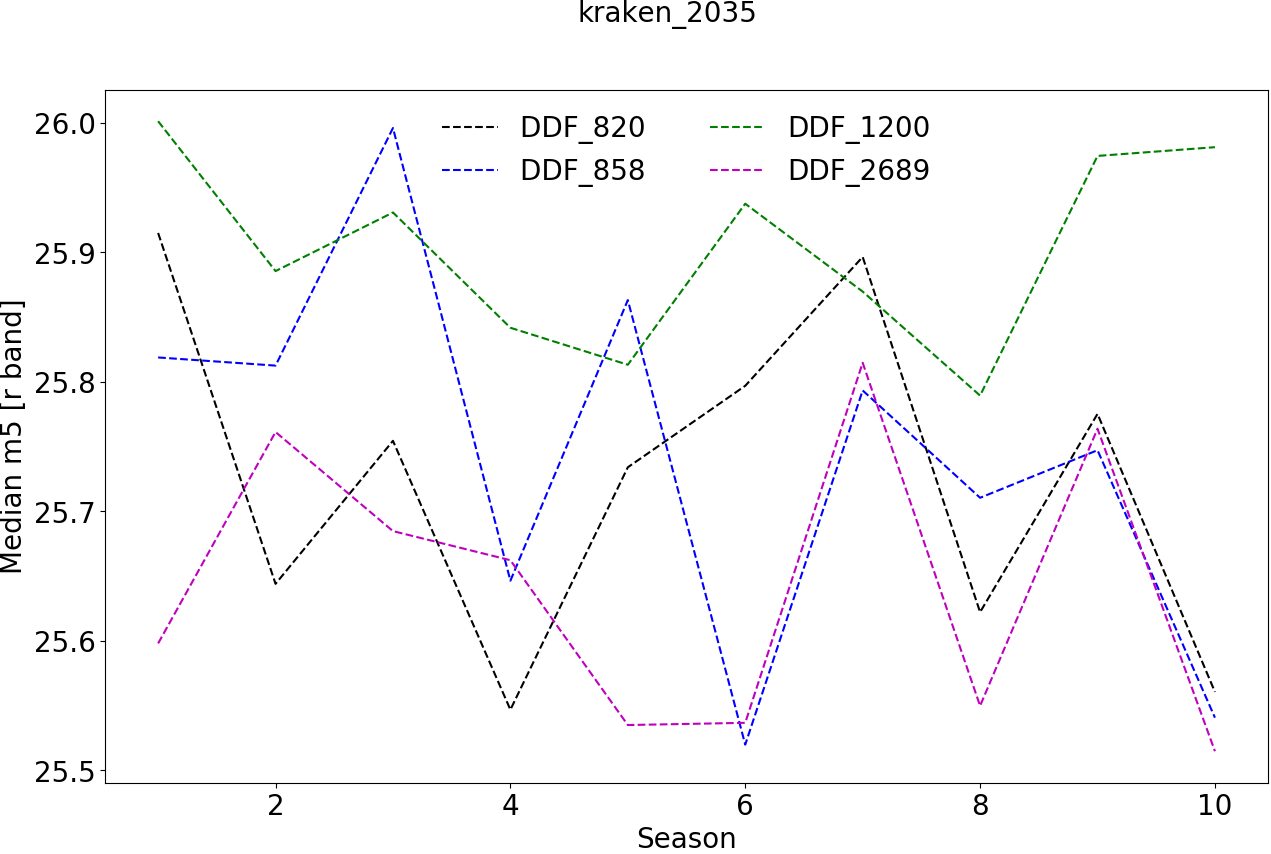
\includegraphics[width=9cm]{overview_strategy/kraken_2035_med_m5.png}
  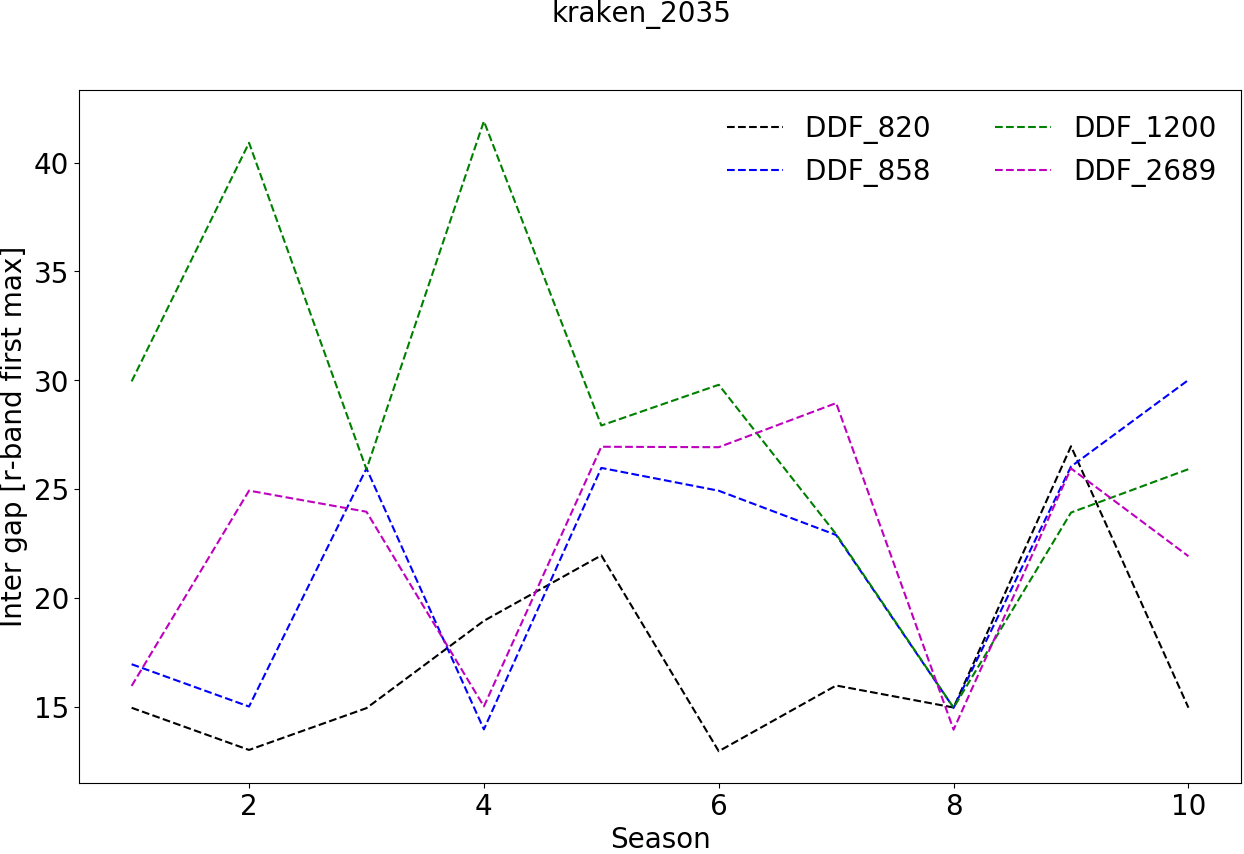
\includegraphics[width=9cm]{overview_strategy/kraken_2035_intergap_max1.png}
    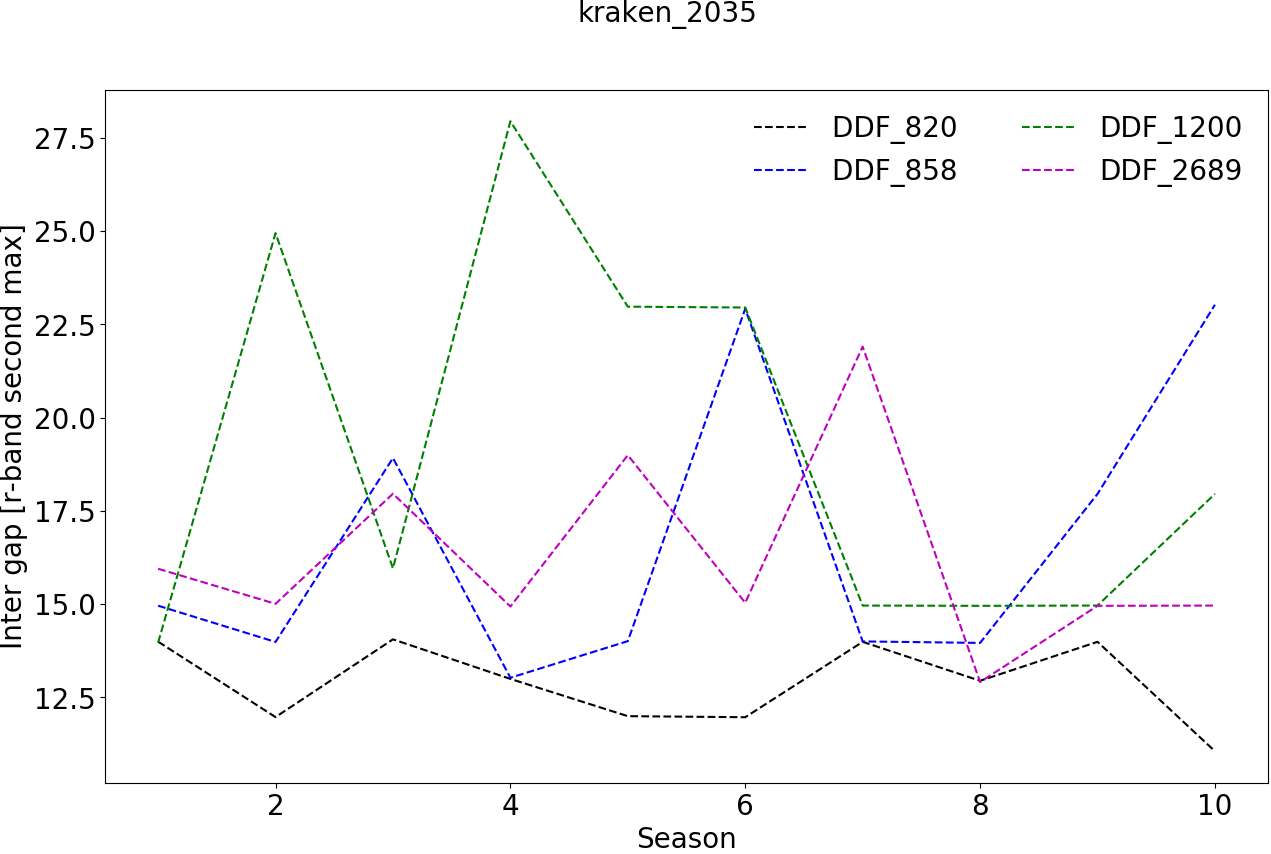
\includegraphics[width=9cm]{overview_strategy/kraken_2035_intergap_max2.png}
    \caption{Median m5 (top, in mag), first maximum inter-night gap (middle, in day) and second maximum inter-night gap (bottom, in day)  as a function of the season for \ddfa, \ddfb, \ddfb and \ddfd fields and kraken\_2035 observing strategy.}\label{fig:kraken_m5}
\end{center}
\end{figure}
